\documentclass[twoside]{article}

% Packages required by doxygen
\usepackage{fixltx2e}
\usepackage{calc}
\usepackage{doxygen}
\usepackage{graphicx}
\usepackage[utf8]{inputenc}
\usepackage{makeidx}
\usepackage{multicol}
\usepackage{multirow}
\PassOptionsToPackage{warn}{textcomp}
\usepackage{textcomp}
\usepackage[nointegrals]{wasysym}
\usepackage[table]{xcolor}

% Font selection
\usepackage[T1]{fontenc}
\usepackage{mathptmx}
\usepackage[scaled=.90]{helvet}
\usepackage{courier}
\usepackage{amssymb}
\usepackage{sectsty}
\renewcommand{\familydefault}{\sfdefault}
\allsectionsfont{%
  \fontseries{bc}\selectfont%
  \color{darkgray}%
}
\renewcommand{\DoxyLabelFont}{%
  \fontseries{bc}\selectfont%
  \color{darkgray}%
}
\newcommand{\+}{\discretionary{\mbox{\scriptsize$\hookleftarrow$}}{}{}}

% Page & text layout
\usepackage[screen]{geometry}
\tolerance=750
\hfuzz=15pt
\hbadness=750
\setlength{\emergencystretch}{15pt}
\setlength{\parindent}{0cm}
\setlength{\parskip}{0.2cm}
\makeatletter
\renewcommand{\paragraph}{%
  \@startsection{paragraph}{4}{0ex}{-1.0ex}{1.0ex}{%
    \normalfont\normalsize\bfseries\SS@parafont%
  }%
}
\renewcommand{\subparagraph}{%
  \@startsection{subparagraph}{5}{0ex}{-1.0ex}{1.0ex}{%
    \normalfont\normalsize\bfseries\SS@subparafont%
  }%
}
\makeatother

% Headers & footers
\usepackage{fancyhdr}
\pagestyle{fancyplain}
\fancyhead[LE]{\fancyplain{}{\bfseries\thepage}}
\fancyhead[CE]{\fancyplain{}{}}
\fancyhead[RE]{\fancyplain{}{\bfseries\leftmark}}
\fancyhead[LO]{\fancyplain{}{\bfseries\rightmark}}
\fancyhead[CO]{\fancyplain{}{}}
\fancyhead[RO]{\fancyplain{}{\bfseries\thepage}}
\fancyfoot[LE]{\fancyplain{}{}}
\fancyfoot[CE]{\fancyplain{}{}}
\fancyfoot[RE]{\fancyplain{}{\bfseries\scriptsize Generated on Fri Dec 8 2017 21\+:02\+:39 for Stock Market -\/ Group Project by Doxygen }}
\fancyfoot[LO]{\fancyplain{}{\bfseries\scriptsize Generated on Fri Dec 8 2017 21\+:02\+:39 for Stock Market -\/ Group Project by Doxygen }}
\fancyfoot[CO]{\fancyplain{}{}}
\fancyfoot[RO]{\fancyplain{}{}}
\renewcommand{\footrulewidth}{0.4pt}
\renewcommand{\sectionmark}[1]{%
  \markright{\thesection\ #1}%
}

% Indices & bibliography
\usepackage{natbib}
\usepackage[titles]{tocloft}
\setcounter{tocdepth}{3}
\setcounter{secnumdepth}{5}
\makeindex

% Packages requested by user
\usepackage{titlesec}

% Hyperlinks (required, but should be loaded last)
\usepackage{ifpdf}
\ifpdf
  \usepackage[pdftex,pagebackref=true]{hyperref}
\else
  \usepackage[ps2pdf,pagebackref=true]{hyperref}
\fi
\hypersetup{%
  colorlinks=true,%
  linkcolor=blue,%
  citecolor=blue,%
  unicode%
}

% Custom commands
\newcommand{\clearemptydoublepage}{%
  \newpage{\pagestyle{empty}\cleardoublepage}%
}


\newcommand{\sectionbreak}{\clearpage}

\begin{document}

% Titlepage & ToC
\hypersetup{pageanchor=false,
             bookmarks=true,
             bookmarksnumbered=true,
             pdfencoding=unicode
            }
\pagenumbering{roman}
\begin{titlepage}
\vspace*{7cm}
\begin{center}%
{\Large Stock Market -\/ Group Project }\\
\vspace*{1cm}
{\large Generated by Doxygen 1.8.8}\\
\vspace*{0.5cm}
{\small Fri Dec 8 2017 21:02:39}\\
\end{center}
\end{titlepage}
\tableofcontents
\pagenumbering{arabic}
\hypersetup{pageanchor=true}

%--- Begin generated contents ---
\section{Specification}
\label{Specification}
\hypertarget{Specification}{}
This program has a built in dictionary for english that can be translated to tagalog. It has a user input in which the user may add the translation of a word that is not within the dictionary. 
\section{Analysis}
\label{Analysis}
\hypertarget{Analysis}{}
inputs will be\+:

\begin{DoxyItemize}
\item The outputs will be\+:\end{DoxyItemize}
\begin{DoxyItemize}
\item The overall algorithim is\+: \end{DoxyItemize}

\section{Design}
\label{Design}
\hypertarget{Design}{}
When this program is launched, the user is given the option to choose from any company they would like do their stock exchange. They are given five different companies in a drop down bar to choose from. Once the user has chosen a company, they are given the option to either sell or buy. After the user has chosen one of those two options, the user is then, asked to give their name, shares amount, and price. After the user has entered the following, the program will then execute and insert the information into the heap tree and search through the heap tree. The heap tree will try to find a matching price that the user has input and it will execute the purchase. If there was no match, it will output \char`\"{}\+No seller/buyer\char`\"{} for the user. Also, if the user enter's the name market, it will purchase/sell the shares from the market. After every purchase and sell, it will display in the live graph and live table. The graph and table will update after every transaction. 
\section{H\+T\+M\+L}
\label{HTML}
\hypertarget{HTML}{}

\begin{DoxyVerbInclude}
<!DOCTYPE html>
<html>
<head>
	<title>cs124 Stockz Lab</title>
  <meta charset="utf-8">
  <meta name="viewport" content="width=device-width, initial-scale=1.0">
  <script type="text/javascript">
  function newData() {
  var dataTable = document.getElementById("dataTable");
  var r = dataTable.insertRow(0);
  var c1 = dataTable.insertRow(0);

  var inputValue = document.getElementById("Stock");
  var strValue = inputValue.options[inputValue.selectedIndex].value;
  
  c1.innerHTML = "hello";
}

function CheckBrowser() {
  if('localStorage' in window && window ['localStorage'] !== null) {
    // we can use local storage
    console.log('local storage works');
    return true;
  }
  else {
    return false;
  }
}

function getStocks(){
  var stocks = new Array;
  var stocks_str= localStorage.getItem('stock');
  console.log(stocks_str);
  if (stocks_str !== null) {
    stocks = JSON.parse(stocks_str);
  }
  return stocks;
}

function getNames(){
  var names = new Array;
  var names_str= localStorage.getItem('name');
  console.log(names_str);
  if (names_str !== null) {
    names = JSON.parse(names_str);
  }
  return names;
}

function getShares(){
  var shares = new Array;
  var shares_str= localStorage.getItem('shares');
  console.log(shares_str);
  if (shares_str !== null) {
    shares = JSON.parse(shares_str);
  }
  return shares;
}

function getTypes(){
  var types = new Array;
  var types_str= localStorage.getItem('type');
  console.log(types_str);
  if (types_str !== null) {
    types = JSON.parse(types_str);
  }
  return types;
}

function getPrices(){
  var prices = new Array;
  var prices_str= localStorage.getItem('price');
  console.log(prices_str);
  if (prices_str !== null) {
    prices = JSON.parse(prices_str);
  }
  return prices;
}

function add() {
  var stock = document.getElementById('Stock').value;

  var stocks = getStocks();
  stocks.push(stock);
  localStorage.setItem('stock', JSON.stringify(stocks));

  var name = document.getElementById('name').value;

  var names = getNames();
  names.push(name);
  localStorage.setItem('name', JSON.stringify(names));

  var share = document.getElementById('shares').value;

  var shares = getShares();
  var shareInt = parseInt(share);
  share = shareInt;
  shares.push(share);
  localStorage.setItem('shares', JSON.stringify(shares));

  var type = document.querySelector('input[name = "o"]:checked').value;

  var types = getTypes();
  types.push(type);
  localStorage.setItem('type', JSON.stringify(types));

  var price = document.getElementById('price').value;
  var priceInt = parseInt(price);
  price = priceInt;
  var prices = getPrices();
  prices.push(price);
  localStorage.setItem('price', JSON.stringify(prices));

  addData();
  show();
}

function show() {
  var stocks = getStocks();
  var names = getNames();
  var shares = getShares();
  var types = getTypes();
  var prices = getPrices();

  /*
  var html = "";
  for ( var i = 0; i <= stocks.length - 1; i++) {
    html += "<tr><td>" + stocks[i] + "</td><td>" + names[i] +
        "</td><td>" + shares[i] + "</td><td>" + types[i] +
        "</td><td>" + prices[i] + "</td></tr>";
  }
  document.getElementById('dataTable').innerHTML = html;
  */
  var table = document.getElementById("dataTable");

  var rowIndex = 1;
  for ( var i = 0; i <= stocks.length - 1; i++) {
    var r = table.insertRow(rowIndex);
    var c1 = r.insertCell(0);
    var c2 = r.insertCell(1);
    var c3 = r.insertCell(2);
    var c4 = r.insertCell(3);
    var c5 = r.insertCell(4);

    c1.innerHTML = stocks[i];
    c2.innerHTML = names[i];
    c3.innerHTML = shares[i];
    c4.innerHTML = types[i];
    c5.innerHTML = prices[i];
    rowIndex++;
  }
}

var dpB = []; // data points Buys
var dpS = []; // data points Sells

function pushData() {
  var types = getTypes();
  var prices = getPrices();
  var shares = getShares();
  for ( var i = dpB.length; i < prices.length; i++ ) {
    var sharesToInt = parseInt(shares[i]);
    var pricesToInt = parseInt(prices[i]);
    if (types[i] == "Buy") {
      dpB.push({
        x: sharesToInt,
        y: pricesToInt
      });
    }
    else if (types[i] == "Sell") {
      dpS.push({
        x: sharesToInt,
        y: pricesToInt
      });
    }
  }
}

function addData() {
  pushData();
  chart.options.data[0].dataPoints = dpB;
  chart.options.data[1].dataPoints = dpS;
  chart.render();
}

var chart;
window.onload = function(){
  CheckBrowser();
  //localStorage.clear();
  chart = new CanvasJS.Chart("chartContainer",
    {
      title:{
      text: "Amazon"  
      },
      data: [
      {        
        type: "bar",
        dataPoints: dpB
      },
      {        
        type: "bar",
        dataPoints: dpS
      }]
    });
    chart.render();
  show();
  addData();
}

//addData();
  </script>
  <script type="text/javascript" src="https://canvasjs.com/assets/script/canvasjs.min.js"></script>
  <link rel="stylesheet" type="text/css" href="main.css">
</head>
<body>
<div class="home">
  <ul class="nav">
    <li><a href="">Home</a></li>
    <li><a href="">Profile</a></li>
    <li><a href="">Trades</a></li>
    <li><a href="">Logout</a></li>
  </ul>
  <h1>Stockz</h1>
  <hr>
  <div class="stockTable-1">
    <h1>EEEE-TRADE</h1>
    <div class="menu">
      <form name=ShoppingMenu action="/cgi-bin/stock">
        <div>
          <label>Choose Stock:</label>
          <select id="Stock" name="Stock">
            <option value="Amazon">Amazon</option>
            <option value="Nvidia">Nvidia</option>
            <option value="BitCoin">BitCoin</option>
            <option value="Ohlone">Ohlone</option>
            <option value="Ganja4Lyfe">Ganja4Lyfe</option>
          </select>
          </div>
        <input type="radio" id="Buy" name="o" value="Buy">Buy
        <input type="radio" id="Sell" name="o" value="Sell">Sell
        <div>
        <label>Name:</label><input type="text" id="name" name="n">
          <div>
            <label>Shares:</label><input type="text" id="shares" name="Z">
          </div>
          <div>
            <label>Price:</label><input type="text" id="price" name="p"><input type="submit" value="Go" onclick="add()">
          </div>
        </div>
      </form>
    </div>
    <div class="stockTable">
      <div id="chartContainer" style="height: 360px; width: 100%;"></div>
    </div>
  </div>
<div class="stockTable">
  <h1>Stock Request</h1>
  <table id="dataTable">
  <tr>
    <th>Stock:</th>
    <th>Name:</th>
    <th>Shares:</th>
    <th>Type:</th>
    <th>Price:</th>
  </tr>
  </table>
</div>
</body>
</html>
\end{DoxyVerbInclude}
 
\section{Images/\+Features}
\label{Images_2Features}
\hypertarget{Images_2Features}{}
In our H\+T\+M\+L, we provided images and features such as a live table and live graph that uses Java\+Script in order to update and show what is added to the Heap. Red bar for sell. Blue bar for buy.

 
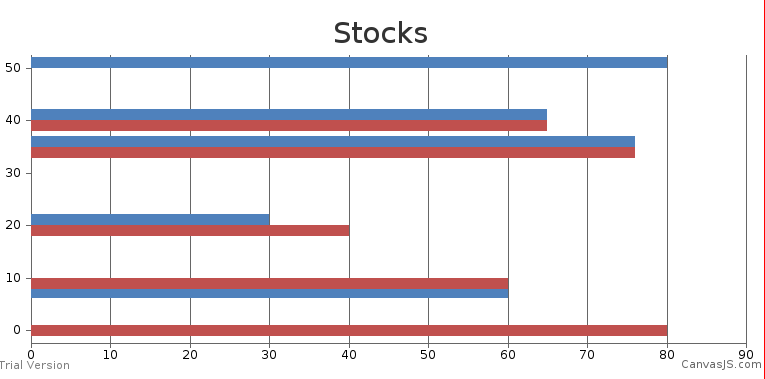
\includegraphics[scale=0.5]{../america.png}
 
\section{Images/\+Features2}
\label{Images_2Features2}
\hypertarget{Images_2Features2}{}
Live Table of Transaction Requests

 
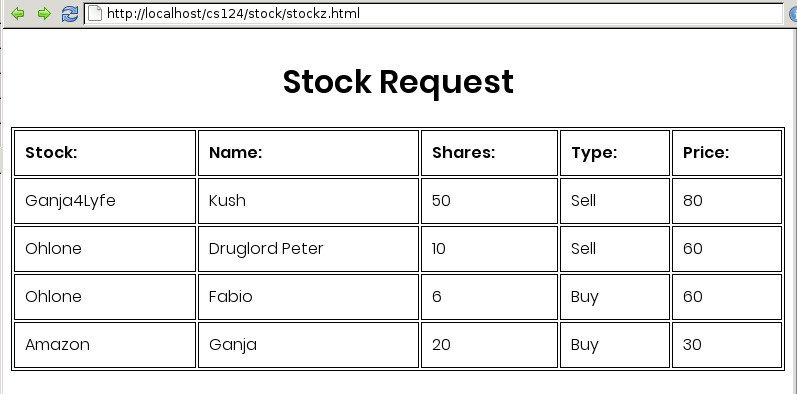
\includegraphics[scale=0.5]{../table.png}
 
\section{Test\+Cases1}
\label{TestCases1}
\hypertarget{TestCases1}{}
Here is our home html page where one can input their name, how many shares, their prices, what stock they like and if they want to buy or sell.

 
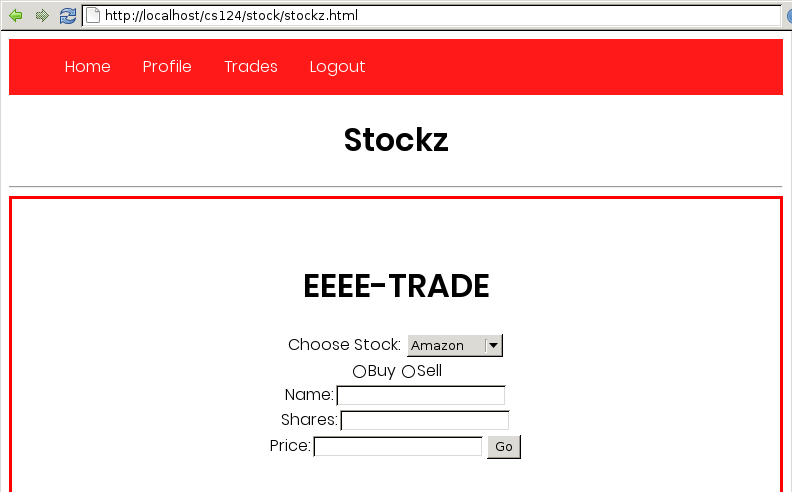
\includegraphics[scale=0.5]{../test1.png}
 
\section{Test\+Cases2}
\label{TestCases2}
\hypertarget{TestCases2}{}
Let's say my buddy Kush wants to sell some of his Amazon stocks, but there are currently no buyers. We would expect that after clicking the go button. We would be redirected to an html page telling us if our transaction went through. Since no one is currently investing in Amazon, we should expect an output saying \char`\"{}no buyer found\char`\"{} and \char`\"{}a request pending\char`\"{}.

 
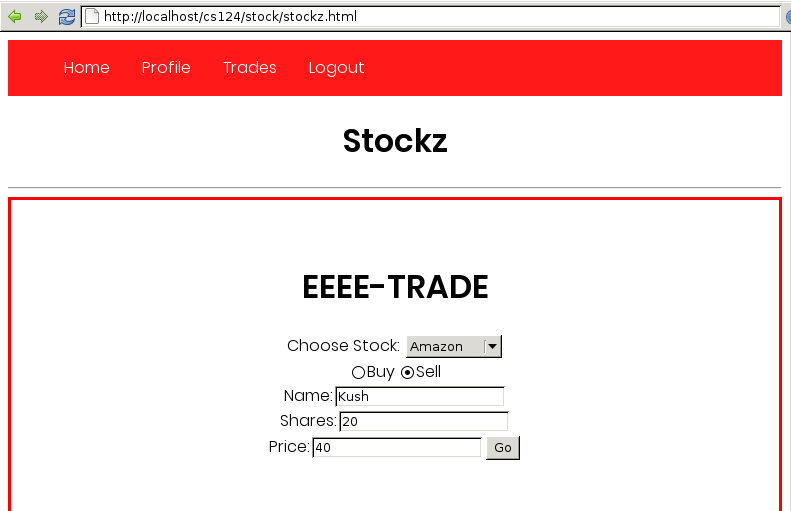
\includegraphics[scale=0.5]{../test2.png}
 
\section{Test\+Cases3}
\label{TestCases3}
\hypertarget{TestCases3}{}
As you can see, after submitting our request, we get our expected output telling us that our request has been added but sadly no one is currently buying.

 
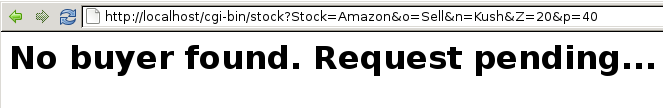
\includegraphics[scale=0.5]{../test3.png}
 
\section{Test\+Cases4}
\label{TestCases4}
\hypertarget{TestCases4}{}
Now don't worry Kush. Although, your request has yet to be fufilled. My buddy Ganja thinks your prices are a bit too much for him and thinks he has a good offer for a lower price. Now when Ganja sends his request, since Kush is the only one selling Amazon stocks but for a higher price. We would expect Ganja to get a similar output but instead it would say that \char`\"{}there are no sellers found and your submission is pending\char`\"{}.

 
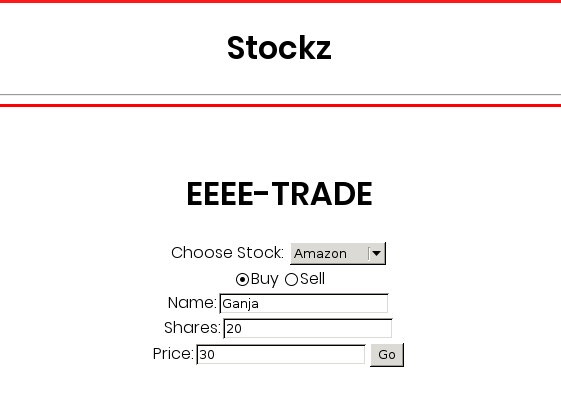
\includegraphics[scale=0.5]{../test4.png}
 
\section{Test\+Cases5}
\label{TestCases5}
\hypertarget{TestCases5}{}
And as expected, Ganja's request has been added, but there is no one selling at that price.

 
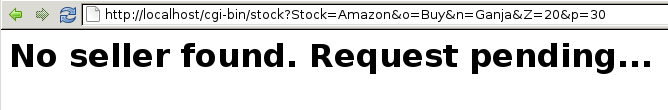
\includegraphics[scale=0.5]{../test5.png}
 
\section{Test\+Case6}
\label{TestCase6}
\hypertarget{TestCase6}{}
Looking at the live graph, Kush sees Ganja's offer and he thinks its a fair deal. So Kush changes his offer to match Ganja's. Now when Kush hits the \char`\"{}go button\char`\"{}, we should expect to see an output saying \char`\"{}there is a match found\char`\"{} and it should display the details of who you are exchanging with. In this case, we should see Ganja's info.

 
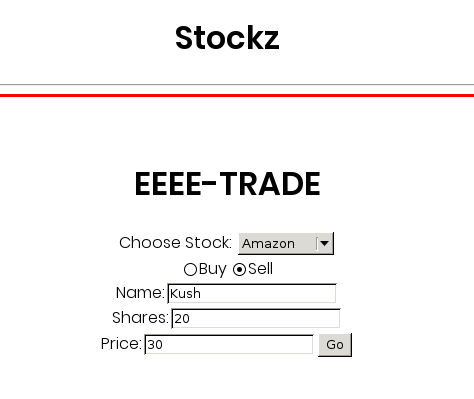
\includegraphics[scale=0.5]{../test6.png}
 
\section{Test\+Case7}
\label{TestCase7}
\hypertarget{TestCase7}{}
Nice! The output is as we expected. We see who we are trading with and the shares they are receiving.

 
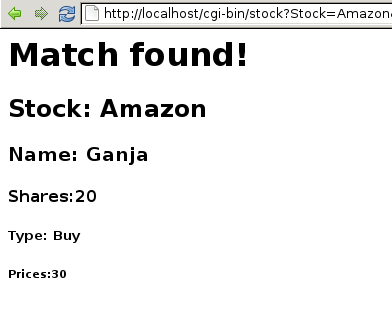
\includegraphics[scale=0.5]{../test7.png}
 
\section{Test\+Case8}
\label{TestCase8}
\hypertarget{TestCase8}{}
Now let's test what happens when there is a partial buy. Here we have Druglord Peter selling 10 Ohlone shares for \$60. Now of course, we need a buyer.

 
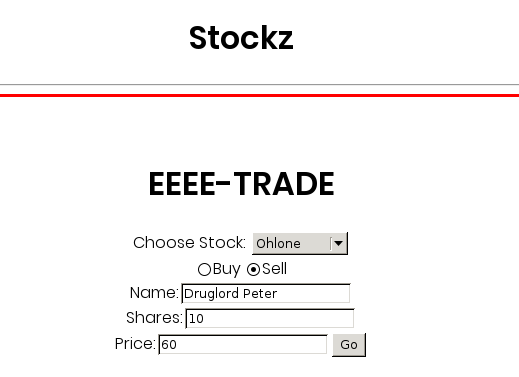
\includegraphics[scale=0.5]{../test8.png}
 
\section{Test\+Case9}
\label{TestCase9}
\hypertarget{TestCase9}{}
Here we have a buyer named Fabio and he only wants 6 Ohlone shares for \$60. When Fabio proceeds, a match would be found and transaction would occur, but O\+N\+L\+Y for those 6 shares.

 
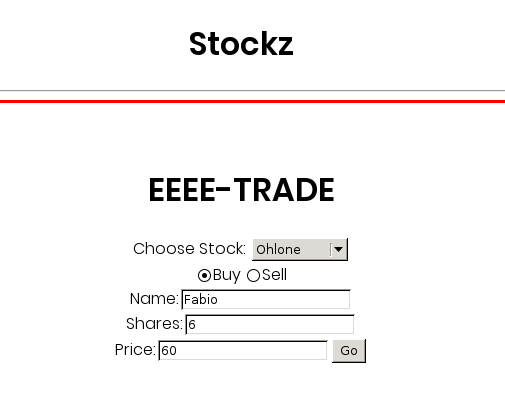
\includegraphics[scale=0.5]{../test9.png}
 
\section{Test\+Case10}
\label{TestCase10}
\hypertarget{TestCase10}{}
Awesome. As expected. We found a match and all information of the other party is displayed and so are the number shares bought.  
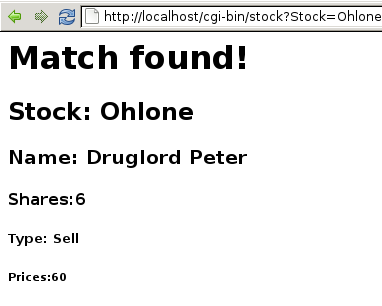
\includegraphics[scale=0.5]{../test10.png}
 
\section{Test\+Case11}
\label{TestCase11}
\hypertarget{TestCase11}{}
Now let's test what happens where there is a partial sell. Here we have Kush again and now he's going to invest all his Amazon earnings on some Ganja4\+Lyfe stocks. He wants 50 shares for \$80. A great deal!

 
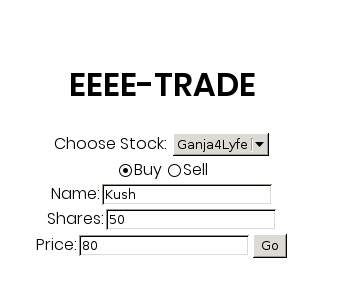
\includegraphics[scale=1.0]{../test11.png}
 
\section{Test\+Case12}
\label{TestCase12}
\hypertarget{TestCase12}{}
And now here we have his old partner Ganja. And he thinks the deal is terrible, but since Kush is such a good sport to sell him those Amazon stocks. He'll sell Kush 1 Ganja4\+Lyfe share. When Ganja submits this request, we should see that there is a match found and the other party's info and the number of stocks exchanged.

 
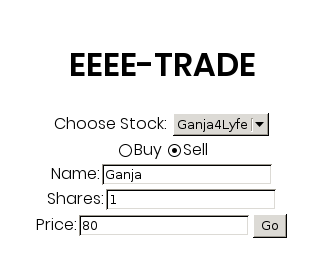
\includegraphics[scale=0.5]{../test13.png}
 
\section{Test\+Case13}
\label{TestCase13}
\hypertarget{TestCase13}{}
Beautiful. As expected, Ganja sells 1 share of Ganja4\+Lyfe to Kush for \$80.

 
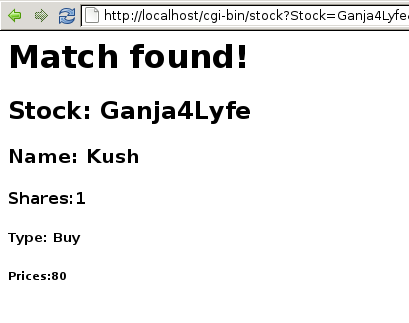
\includegraphics[scale=0.5]{../test14.png}
 
\section{Test\+Case14}
\label{TestCase14}
\hypertarget{TestCase14}{}
Now let's try to do a market sell. We should see a successful transaction, since the market handles the request.

 
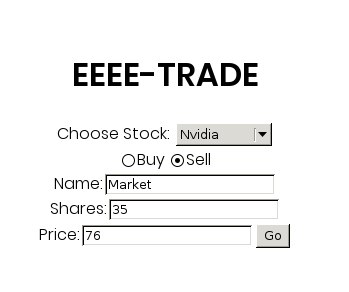
\includegraphics[scale=0.5]{../test15.png}
 
\section{Test\+Case15}
\label{TestCase15}
\hypertarget{TestCase15}{}
Nice!

 
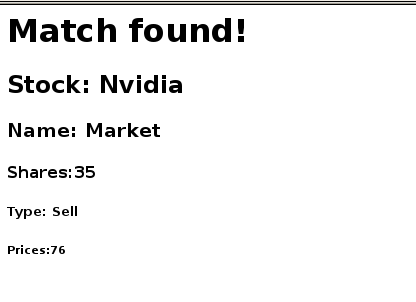
\includegraphics[scale=0.5]{../test16.png}
 
\section{Test\+Case16}
\label{TestCase16}
\hypertarget{TestCase16}{}
How about market buy? The same should happen.

 
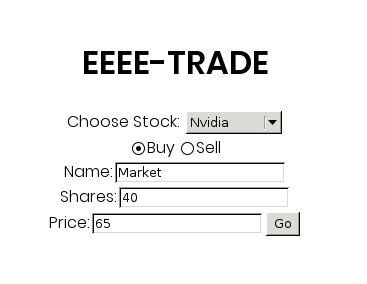
\includegraphics[scale=0.5]{../test17.png}
 
\section{Test\+Case17}
\label{TestCase17}
\hypertarget{TestCase17}{}
Market buy works too!

 
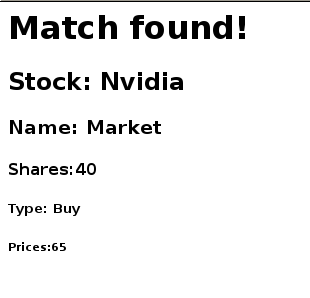
\includegraphics[scale=0.5]{../test18.png}
 
\section{Class Index}
\subsection{Class List}
Here are the classes, structs, unions and interfaces with brief descriptions\+:\begin{DoxyCompactList}
\item\contentsline{section}{\hyperlink{structENTRY}{E\+N\+T\+R\+Y} }{\pageref{structENTRY}}{}
\end{DoxyCompactList}

\section{File Index}
\subsection{File List}
Here is a list of all files with brief descriptions\+:\begin{DoxyCompactList}
\item\contentsline{section}{\hyperlink{BuildListDirectly_8cpp}{Build\+List\+Directly.\+cpp} }{\pageref{BuildListDirectly_8cpp}}{}
\item\contentsline{section}{\hyperlink{destroyList_8cpp}{destroy\+List.\+cpp} }{\pageref{destroyList_8cpp}}{}
\item\contentsline{section}{\hyperlink{displayList_8cpp}{display\+List.\+cpp} }{\pageref{displayList_8cpp}}{}
\item\contentsline{section}{\hyperlink{Insert_8cpp}{Insert.\+cpp} }{\pageref{Insert_8cpp}}{}
\item\contentsline{section}{\hyperlink{InsertInOrder_8cpp}{Insert\+In\+Order.\+cpp} }{\pageref{InsertInOrder_8cpp}}{}
\item\contentsline{section}{\hyperlink{lab2_8h}{lab2.\+h} }{\pageref{lab2_8h}}{}
\item\contentsline{section}{\hyperlink{loadList_8cpp}{load\+List.\+cpp} }{\pageref{loadList_8cpp}}{}
\item\contentsline{section}{\hyperlink{loadList2_8cpp}{load\+List2.\+cpp} }{\pageref{loadList2_8cpp}}{}
\item\contentsline{section}{\hyperlink{loadList3_8cpp}{load\+List3.\+cpp} }{\pageref{loadList3_8cpp}}{}
\item\contentsline{section}{\hyperlink{main_8cpp}{main.\+cpp} }{\pageref{main_8cpp}}{}
\end{DoxyCompactList}

\section{Class Documentation}
\hypertarget{classHEAP}{\subsection{H\+E\+A\+P$<$ S\+O\+M\+E\+T\+Y\+P\+E $>$ Class Template Reference}
\label{classHEAP}\index{H\+E\+A\+P$<$ S\+O\+M\+E\+T\+Y\+P\+E $>$@{H\+E\+A\+P$<$ S\+O\+M\+E\+T\+Y\+P\+E $>$}}
}


This is a class \hyperlink{classHEAP}{H\+E\+A\+P} which includes all function and storage needed to make the program and tree.  




{\ttfamily \#include $<$H\+E\+A\+P.\+H$>$}



Collaboration diagram for H\+E\+A\+P$<$ S\+O\+M\+E\+T\+Y\+P\+E $>$\+:\nopagebreak
\begin{figure}[H]
\begin{center}
\leavevmode
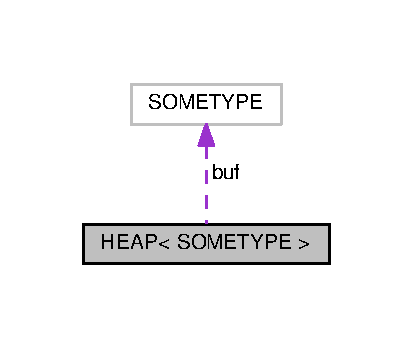
\includegraphics[width=198pt]{classHEAP__coll__graph}
\end{center}
\end{figure}
\subsubsection*{Public Types}
\begin{DoxyCompactItemize}
\item 
enum \hyperlink{classHEAP_a440ecc6b7771102dbaa63b3dacce6c27}{heap\+Type} \{ \hyperlink{classHEAP_a440ecc6b7771102dbaa63b3dacce6c27af40ccc5dc19d4acb72467707512926c6}{M\+A\+X}, 
\hyperlink{classHEAP_a440ecc6b7771102dbaa63b3dacce6c27a38253c74a285d04166dcc555cb4c8f19}{M\+I\+N}
 \}
\end{DoxyCompactItemize}
\subsubsection*{Public Member Functions}
\begin{DoxyCompactItemize}
\item 
\hyperlink{classHEAP_a341e0d88f79b41d55f804b759646d13c}{H\+E\+A\+P} (int a\+\_\+size, \hyperlink{classHEAP_a440ecc6b7771102dbaa63b3dacce6c27}{heap\+Type})
\begin{DoxyCompactList}\small\item\em This is a constructor which build a heap tree of size a\+\_\+size. \end{DoxyCompactList}\item 
\hyperlink{classHEAP_a7a99ff54ff586bbee33e36828bb7a2f7}{$\sim$\+H\+E\+A\+P} ()
\begin{DoxyCompactList}\small\item\em This is a destructor to destroy the heap trees. \end{DoxyCompactList}\item 
bool \hyperlink{classHEAP_a560500cc8aa1dc1d07dbc4e6c4d1b5f3}{Is\+Empty} ()
\item 
bool \hyperlink{classHEAP_ac2560a1c0edc4cecc583880fe6006a91}{Is\+Full} ()
\item 
\hyperlink{HEAP_8H_a32c27cc471df37f4fc818d65de0a56c4}{S\+T\+A\+T\+U\+S} \hyperlink{classHEAP_a61daf2c080cdb92947a0e591fbd8d772}{Insert} (S\+O\+M\+E\+T\+Y\+P\+E x)
\begin{DoxyCompactList}\small\item\em This is a insert function to add data into the heap trees. \end{DoxyCompactList}\item 
\hyperlink{HEAP_8H_a32c27cc471df37f4fc818d65de0a56c4}{S\+T\+A\+T\+U\+S} \hyperlink{classHEAP_aedf7ac5c115a4d0bb96139da8788f26a}{Remove} (S\+O\+M\+E\+T\+Y\+P\+E \&x)
\begin{DoxyCompactList}\small\item\em This is a remove function to remove data from the heap trees. \end{DoxyCompactList}\item 
void \hyperlink{classHEAP_a07fcd2f8486f24a64f216a7c2bfdbf77}{print\+Heap} ()
\begin{DoxyCompactList}\small\item\em This is a function that prints out the heap tree. \end{DoxyCompactList}\item 
void \hyperlink{classHEAP_a935705273d6321f27ff5e73f6a86f220}{add\+Max\+H\+V} (int value)
\item 
void \hyperlink{classHEAP_a49697dff68d8383e2aec0cd757fd4201}{push\+Max\+Heap\+Data} ()
\begin{DoxyCompactList}\small\item\em This is a push function that pushes information from max\+Heap into a vector. \end{DoxyCompactList}\item 
void \hyperlink{classHEAP_a60ee205bf01ba40b2de104f9058e612f}{display\+Vector} ()
\item 
void \hyperlink{classHEAP_a3c1097a2a0b425a08a8da33c2c35edf7}{temp\+Max\+Heap} ()
\begin{DoxyCompactList}\small\item\em This is a funcction that adds the information from max\+Heap into a temp vector. \end{DoxyCompactList}\item 
void \hyperlink{classHEAP_a5985dc9dbed06ce7aa3899b40ab80134}{temp\+Min\+Heap} ()
\begin{DoxyCompactList}\small\item\em This is a function that adds the information from min\+Heap into a temp vector. \end{DoxyCompactList}\end{DoxyCompactItemize}
\subsubsection*{Public Attributes}
\begin{DoxyCompactItemize}
\item 
S\+O\+M\+E\+T\+Y\+P\+E $\ast$ \hyperlink{classHEAP_abe5af2e4e8f2bc55e5b2e70ffa43e630}{buf}
\item 
int \hyperlink{classHEAP_a660f8fd84a9646a631badb8c6ca87aca}{size}
\item 
int \hyperlink{classHEAP_ad481b16366a0a0ff65418afc71d9e652}{n\+Nodes}
\item 
std\+::vector$<$ int $>$ \hyperlink{classHEAP_a541eab0dba5cd90e27be6083b1a1979f}{min\+H\+V}
\item 
std\+::vector$<$ int $>$ \hyperlink{classHEAP_a33776b33a838c2116349c676ac2a7249}{max\+H\+V}
\item 
std\+::vector$<$ int $>$ \hyperlink{classHEAP_adc22726c34c72025819274f63d8bb418}{index\+Min\+H\+V}
\item 
std\+::vector$<$ int $>$ \hyperlink{classHEAP_af6c485575f29a80d91f611af87b7f6b8}{index\+Max\+H\+V}
\item 
int \hyperlink{classHEAP_a82daf731595f82a6224fc9360b63a58d}{temp\+Max\+V}
\item 
int \hyperlink{classHEAP_a0402f157889d6b40f219c608bc9a3503}{temp\+Min\+V}
\end{DoxyCompactItemize}


\subsubsection{Detailed Description}
\subsubsection*{template$<$class S\+O\+M\+E\+T\+Y\+P\+E$>$class H\+E\+A\+P$<$ S\+O\+M\+E\+T\+Y\+P\+E $>$}

This is a class \hyperlink{classHEAP}{H\+E\+A\+P} which includes all function and storage needed to make the program and tree. 

\subsubsection{Member Enumeration Documentation}
\hypertarget{classHEAP_a440ecc6b7771102dbaa63b3dacce6c27}{\index{H\+E\+A\+P@{H\+E\+A\+P}!heap\+Type@{heap\+Type}}
\index{heap\+Type@{heap\+Type}!H\+E\+A\+P@{H\+E\+A\+P}}
\paragraph[{heap\+Type}]{\setlength{\rightskip}{0pt plus 5cm}template$<$class S\+O\+M\+E\+T\+Y\+P\+E$>$ enum {\bf H\+E\+A\+P\+::heap\+Type}}}\label{classHEAP_a440ecc6b7771102dbaa63b3dacce6c27}
\begin{Desc}
\item[Enumerator]\par
\begin{description}
\index{M\+A\+X@{M\+A\+X}!H\+E\+A\+P@{H\+E\+A\+P}}\index{H\+E\+A\+P@{H\+E\+A\+P}!M\+A\+X@{M\+A\+X}}\item[{\em 
\hypertarget{classHEAP_a440ecc6b7771102dbaa63b3dacce6c27af40ccc5dc19d4acb72467707512926c6}{M\+A\+X}\label{classHEAP_a440ecc6b7771102dbaa63b3dacce6c27af40ccc5dc19d4acb72467707512926c6}
}]\index{M\+I\+N@{M\+I\+N}!H\+E\+A\+P@{H\+E\+A\+P}}\index{H\+E\+A\+P@{H\+E\+A\+P}!M\+I\+N@{M\+I\+N}}\item[{\em 
\hypertarget{classHEAP_a440ecc6b7771102dbaa63b3dacce6c27a38253c74a285d04166dcc555cb4c8f19}{M\+I\+N}\label{classHEAP_a440ecc6b7771102dbaa63b3dacce6c27a38253c74a285d04166dcc555cb4c8f19}
}]\end{description}
\end{Desc}

\begin{DoxyCode}
26 \{\hyperlink{classHEAP_a440ecc6b7771102dbaa63b3dacce6c27af40ccc5dc19d4acb72467707512926c6}{MAX},\hyperlink{classHEAP_a440ecc6b7771102dbaa63b3dacce6c27a38253c74a285d04166dcc555cb4c8f19}{MIN}\};
\end{DoxyCode}


\subsubsection{Constructor \& Destructor Documentation}
\hypertarget{classHEAP_a341e0d88f79b41d55f804b759646d13c}{\index{H\+E\+A\+P@{H\+E\+A\+P}!H\+E\+A\+P@{H\+E\+A\+P}}
\index{H\+E\+A\+P@{H\+E\+A\+P}!H\+E\+A\+P@{H\+E\+A\+P}}
\paragraph[{H\+E\+A\+P}]{\setlength{\rightskip}{0pt plus 5cm}template$<$class S\+O\+M\+E\+T\+Y\+P\+E $>$ {\bf H\+E\+A\+P}$<$ S\+O\+M\+E\+T\+Y\+P\+E $>$\+::{\bf H\+E\+A\+P} (
\begin{DoxyParamCaption}
\item[{int}]{a\+\_\+size, }
\item[{{\bf heap\+Type}}]{ht}
\end{DoxyParamCaption}
)}}\label{classHEAP_a341e0d88f79b41d55f804b759646d13c}


This is a constructor which build a heap tree of size a\+\_\+size. 


\begin{DoxyParams}{Parameters}
{\em a\+\_\+size} & declares the size of the heap tree and which type of heap tree it will become \\
\hline
\end{DoxyParams}

\begin{DoxyCode}
117 \{
118     t = ht;
119     \hyperlink{classHEAP_ad481b16366a0a0ff65418afc71d9e652}{nNodes} = 0;
120     \hyperlink{classHEAP_abe5af2e4e8f2bc55e5b2e70ffa43e630}{buf} = \textcolor{keyword}{new} SOMETYPE[a\_size+1]; \textcolor{comment}{// +1 because buf[0] is not used}
121     \textcolor{keywordflow}{if} (\hyperlink{classHEAP_abe5af2e4e8f2bc55e5b2e70ffa43e630}{buf}) \hyperlink{classHEAP_a660f8fd84a9646a631badb8c6ca87aca}{size} = a\_size;
122     \textcolor{keywordflow}{else} \hyperlink{classHEAP_a660f8fd84a9646a631badb8c6ca87aca}{size} = 0;
123 \}
\end{DoxyCode}
\hypertarget{classHEAP_a7a99ff54ff586bbee33e36828bb7a2f7}{\index{H\+E\+A\+P@{H\+E\+A\+P}!````~H\+E\+A\+P@{$\sim$\+H\+E\+A\+P}}
\index{````~H\+E\+A\+P@{$\sim$\+H\+E\+A\+P}!H\+E\+A\+P@{H\+E\+A\+P}}
\paragraph[{$\sim$\+H\+E\+A\+P}]{\setlength{\rightskip}{0pt plus 5cm}template$<$class S\+O\+M\+E\+T\+Y\+P\+E $>$ {\bf H\+E\+A\+P}$<$ S\+O\+M\+E\+T\+Y\+P\+E $>$\+::$\sim${\bf H\+E\+A\+P} (
\begin{DoxyParamCaption}
{}
\end{DoxyParamCaption}
)}}\label{classHEAP_a7a99ff54ff586bbee33e36828bb7a2f7}


This is a destructor to destroy the heap trees. 


\begin{DoxyCode}
134 \{
135     \textcolor{keyword}{delete} [] \hyperlink{classHEAP_abe5af2e4e8f2bc55e5b2e70ffa43e630}{buf};
136 \}
\end{DoxyCode}


\subsubsection{Member Function Documentation}
\hypertarget{classHEAP_a935705273d6321f27ff5e73f6a86f220}{\index{H\+E\+A\+P@{H\+E\+A\+P}!add\+Max\+H\+V@{add\+Max\+H\+V}}
\index{add\+Max\+H\+V@{add\+Max\+H\+V}!H\+E\+A\+P@{H\+E\+A\+P}}
\paragraph[{add\+Max\+H\+V}]{\setlength{\rightskip}{0pt plus 5cm}template$<$class S\+O\+M\+E\+T\+Y\+P\+E$>$ void {\bf H\+E\+A\+P}$<$ S\+O\+M\+E\+T\+Y\+P\+E $>$\+::add\+Max\+H\+V (
\begin{DoxyParamCaption}
\item[{int}]{value}
\end{DoxyParamCaption}
)}}\label{classHEAP_a935705273d6321f27ff5e73f6a86f220}
\hypertarget{classHEAP_a60ee205bf01ba40b2de104f9058e612f}{\index{H\+E\+A\+P@{H\+E\+A\+P}!display\+Vector@{display\+Vector}}
\index{display\+Vector@{display\+Vector}!H\+E\+A\+P@{H\+E\+A\+P}}
\paragraph[{display\+Vector}]{\setlength{\rightskip}{0pt plus 5cm}template$<$class S\+O\+M\+E\+T\+Y\+P\+E$>$ void {\bf H\+E\+A\+P}$<$ S\+O\+M\+E\+T\+Y\+P\+E $>$\+::display\+Vector (
\begin{DoxyParamCaption}
{}
\end{DoxyParamCaption}
)}}\label{classHEAP_a60ee205bf01ba40b2de104f9058e612f}
\hypertarget{classHEAP_a61daf2c080cdb92947a0e591fbd8d772}{\index{H\+E\+A\+P@{H\+E\+A\+P}!Insert@{Insert}}
\index{Insert@{Insert}!H\+E\+A\+P@{H\+E\+A\+P}}
\paragraph[{Insert}]{\setlength{\rightskip}{0pt plus 5cm}template$<$class S\+O\+M\+E\+T\+Y\+P\+E$>$ {\bf S\+T\+A\+T\+U\+S} {\bf H\+E\+A\+P}$<$ S\+O\+M\+E\+T\+Y\+P\+E $>$\+::Insert (
\begin{DoxyParamCaption}
\item[{S\+O\+M\+E\+T\+Y\+P\+E}]{x}
\end{DoxyParamCaption}
)}}\label{classHEAP_a61daf2c080cdb92947a0e591fbd8d772}


This is a insert function to add data into the heap trees. 


\begin{DoxyParams}{Parameters}
{\em sometype} & which is basically an int of x \\
\hline
\end{DoxyParams}
\begin{DoxyReturn}{Returns}
returns O\+K 
\end{DoxyReturn}

\begin{DoxyCode}
150 \{
151     \textcolor{keywordflow}{if} (\hyperlink{classHEAP_ac2560a1c0edc4cecc583880fe6006a91}{IsFull}()) \textcolor{keywordflow}{return} \hyperlink{HEAP_8H_a32c27cc471df37f4fc818d65de0a56c4aecedb56d1405a60c6069f4a0139bdec5}{FAILED};
152 
153     \hyperlink{classHEAP_ad481b16366a0a0ff65418afc71d9e652}{nNodes}++;  \textcolor{comment}{// The last node of the heap is now vacant.}
154 
155     \textcolor{comment}{// Starting from the (vacant) last node, go from node i to}
156     \textcolor{comment}{//   its parent iParent and, }
157     
158     \textcolor{comment}{// if it is a max heap then as long as the parent is smaller }
159     \textcolor{comment}{//  than x, move the parent down:}
160     \textcolor{comment}{// if it is a min heap then as long as the parent is }
161     \textcolor{comment}{//  larger than x, move the x up:}
162 
163     \textcolor{keywordtype}{int} i = \hyperlink{classHEAP_ad481b16366a0a0ff65418afc71d9e652}{nNodes};
164     \textcolor{keywordtype}{int} iParent;
165     \textcolor{keywordflow}{while} (i > 1) \{
166         iParent = i/2;
167         
168         \textcolor{keywordflow}{if}(t == \hyperlink{classHEAP_a440ecc6b7771102dbaa63b3dacce6c27af40ccc5dc19d4acb72467707512926c6}{MAX})
169         \{
170             \textcolor{keywordflow}{if} (x <= \hyperlink{classHEAP_abe5af2e4e8f2bc55e5b2e70ffa43e630}{buf}[iParent]) \textcolor{keywordflow}{break};
171         \}
172         \textcolor{keywordflow}{else} \textcolor{comment}{// must be MIN}
173         \{
174             \textcolor{keywordflow}{if}( x >= \hyperlink{classHEAP_abe5af2e4e8f2bc55e5b2e70ffa43e630}{buf}[iParent]) \textcolor{keywordflow}{break};
175         \}
176         \hyperlink{classHEAP_abe5af2e4e8f2bc55e5b2e70ffa43e630}{buf}[i] = \hyperlink{classHEAP_abe5af2e4e8f2bc55e5b2e70ffa43e630}{buf}[iParent];
177         i = iParent;
178     \}
179 
180     \textcolor{comment}{// Insert x into the created vacancy:}
181     \hyperlink{classHEAP_abe5af2e4e8f2bc55e5b2e70ffa43e630}{buf}[i] = x;
182 
183     \textcolor{keywordflow}{return} \hyperlink{HEAP_8H_a32c27cc471df37f4fc818d65de0a56c4a2bc49ec37d6a5715dd23e85f1ff5bb59}{OK};
184 \}
\end{DoxyCode}
\hypertarget{classHEAP_a560500cc8aa1dc1d07dbc4e6c4d1b5f3}{\index{H\+E\+A\+P@{H\+E\+A\+P}!Is\+Empty@{Is\+Empty}}
\index{Is\+Empty@{Is\+Empty}!H\+E\+A\+P@{H\+E\+A\+P}}
\paragraph[{Is\+Empty}]{\setlength{\rightskip}{0pt plus 5cm}template$<$class S\+O\+M\+E\+T\+Y\+P\+E$>$ bool {\bf H\+E\+A\+P}$<$ S\+O\+M\+E\+T\+Y\+P\+E $>$\+::Is\+Empty (
\begin{DoxyParamCaption}
{}
\end{DoxyParamCaption}
)\hspace{0.3cm}{\ttfamily [inline]}}}\label{classHEAP_a560500cc8aa1dc1d07dbc4e6c4d1b5f3}

\begin{DoxyCode}
45 \{\textcolor{keywordflow}{return} (\hyperlink{classHEAP_ad481b16366a0a0ff65418afc71d9e652}{nNodes} == 0);\}
\end{DoxyCode}
\hypertarget{classHEAP_ac2560a1c0edc4cecc583880fe6006a91}{\index{H\+E\+A\+P@{H\+E\+A\+P}!Is\+Full@{Is\+Full}}
\index{Is\+Full@{Is\+Full}!H\+E\+A\+P@{H\+E\+A\+P}}
\paragraph[{Is\+Full}]{\setlength{\rightskip}{0pt plus 5cm}template$<$class S\+O\+M\+E\+T\+Y\+P\+E$>$ bool {\bf H\+E\+A\+P}$<$ S\+O\+M\+E\+T\+Y\+P\+E $>$\+::Is\+Full (
\begin{DoxyParamCaption}
{}
\end{DoxyParamCaption}
)\hspace{0.3cm}{\ttfamily [inline]}}}\label{classHEAP_ac2560a1c0edc4cecc583880fe6006a91}

\begin{DoxyCode}
46 \{\textcolor{keywordflow}{return} (\hyperlink{classHEAP_ad481b16366a0a0ff65418afc71d9e652}{nNodes} == \hyperlink{classHEAP_a660f8fd84a9646a631badb8c6ca87aca}{size});\}
\end{DoxyCode}
\hypertarget{classHEAP_a07fcd2f8486f24a64f216a7c2bfdbf77}{\index{H\+E\+A\+P@{H\+E\+A\+P}!print\+Heap@{print\+Heap}}
\index{print\+Heap@{print\+Heap}!H\+E\+A\+P@{H\+E\+A\+P}}
\paragraph[{print\+Heap}]{\setlength{\rightskip}{0pt plus 5cm}template$<$class S\+O\+M\+E\+T\+Y\+P\+E $>$ void {\bf H\+E\+A\+P}$<$ S\+O\+M\+E\+T\+Y\+P\+E $>$\+::print\+Heap (
\begin{DoxyParamCaption}
{}
\end{DoxyParamCaption}
)}}\label{classHEAP_a07fcd2f8486f24a64f216a7c2bfdbf77}


This is a function that prints out the heap tree. 


\begin{DoxyCode}
64 \{
65     \textcolor{keywordflow}{for}(\textcolor{keywordtype}{int} i = 1; i < \hyperlink{classHEAP_ad481b16366a0a0ff65418afc71d9e652}{nNodes}; i++)
66         std::cout << \hyperlink{classHEAP_abe5af2e4e8f2bc55e5b2e70ffa43e630}{buf}[i] << std::endl;
67 \}
\end{DoxyCode}
\hypertarget{classHEAP_a49697dff68d8383e2aec0cd757fd4201}{\index{H\+E\+A\+P@{H\+E\+A\+P}!push\+Max\+Heap\+Data@{push\+Max\+Heap\+Data}}
\index{push\+Max\+Heap\+Data@{push\+Max\+Heap\+Data}!H\+E\+A\+P@{H\+E\+A\+P}}
\paragraph[{push\+Max\+Heap\+Data}]{\setlength{\rightskip}{0pt plus 5cm}template$<$class S\+O\+M\+E\+T\+Y\+P\+E $>$ void {\bf H\+E\+A\+P}$<$ S\+O\+M\+E\+T\+Y\+P\+E $>$\+::push\+Max\+Heap\+Data (
\begin{DoxyParamCaption}
{}
\end{DoxyParamCaption}
)}}\label{classHEAP_a49697dff68d8383e2aec0cd757fd4201}


This is a push function that pushes information from max\+Heap into a vector. 


\begin{DoxyCode}
103 \{
104     \textcolor{keywordflow}{for}(\textcolor{keywordtype}{int} i = 1; i < \hyperlink{classHEAP_ad481b16366a0a0ff65418afc71d9e652}{nNodes}; i++)
105         \hyperlink{classHEAP_a33776b33a838c2116349c676ac2a7249}{maxHV}.push\_back(\hyperlink{classHEAP_abe5af2e4e8f2bc55e5b2e70ffa43e630}{buf}[i]);
106 \}
\end{DoxyCode}
\hypertarget{classHEAP_aedf7ac5c115a4d0bb96139da8788f26a}{\index{H\+E\+A\+P@{H\+E\+A\+P}!Remove@{Remove}}
\index{Remove@{Remove}!H\+E\+A\+P@{H\+E\+A\+P}}
\paragraph[{Remove}]{\setlength{\rightskip}{0pt plus 5cm}template$<$class S\+O\+M\+E\+T\+Y\+P\+E$>$ {\bf S\+T\+A\+T\+U\+S} {\bf H\+E\+A\+P}$<$ S\+O\+M\+E\+T\+Y\+P\+E $>$\+::Remove (
\begin{DoxyParamCaption}
\item[{S\+O\+M\+E\+T\+Y\+P\+E \&}]{x}
\end{DoxyParamCaption}
)}}\label{classHEAP_aedf7ac5c115a4d0bb96139da8788f26a}


This is a remove function to remove data from the heap trees. 


\begin{DoxyParams}{Parameters}
{\em sometype} & which is basically an int reference of x \\
\hline
\end{DoxyParams}
\begin{DoxyReturn}{Returns}
returns O\+K 
\end{DoxyReturn}

\begin{DoxyCode}
199 \{
200     \textcolor{keywordflow}{if} (\hyperlink{classHEAP_a560500cc8aa1dc1d07dbc4e6c4d1b5f3}{IsEmpty}()) \textcolor{keywordflow}{return} \hyperlink{HEAP_8H_a32c27cc471df37f4fc818d65de0a56c4aecedb56d1405a60c6069f4a0139bdec5}{FAILED};
201 
202     \textcolor{comment}{// Retrieve the top element:}
203 
204     x = \hyperlink{classHEAP_abe5af2e4e8f2bc55e5b2e70ffa43e630}{buf}[1];             
205 
206     \textcolor{comment}{// Starting from the vacant root, go from node iParent to its}
207     \textcolor{comment}{//   larger child i and, as long as that child}
208     \textcolor{comment}{//   is greater than the last element of the heap,}
209     \textcolor{comment}{//   move that child up:}
210 
211     \textcolor{keywordtype}{int} iParent = 1;       \textcolor{comment}{// root}
212     \textcolor{keywordtype}{int} i = 2;             \textcolor{comment}{// its left child}
213     \textcolor{keywordflow}{while} (i <= \hyperlink{classHEAP_ad481b16366a0a0ff65418afc71d9e652}{nNodes}) \{
214         \textcolor{comment}{// Set i to the right child, i+1, if it}
215         \textcolor{comment}{//   exists and is larger:}
216         \textcolor{keywordflow}{if} (i < \hyperlink{classHEAP_ad481b16366a0a0ff65418afc71d9e652}{nNodes} && \hyperlink{classHEAP_abe5af2e4e8f2bc55e5b2e70ffa43e630}{buf}[i] < \hyperlink{classHEAP_abe5af2e4e8f2bc55e5b2e70ffa43e630}{buf}[i+1]) i++;
217         \textcolor{keywordflow}{if} (t == \hyperlink{classHEAP_a440ecc6b7771102dbaa63b3dacce6c27a38253c74a285d04166dcc555cb4c8f19}{MIN})
218             \textcolor{keywordflow}{if}(i < \hyperlink{classHEAP_ad481b16366a0a0ff65418afc71d9e652}{nNodes} && \hyperlink{classHEAP_abe5af2e4e8f2bc55e5b2e70ffa43e630}{buf}[i] > \hyperlink{classHEAP_abe5af2e4e8f2bc55e5b2e70ffa43e630}{buf}[i+1]) i++;
219         \textcolor{keywordflow}{if} (t == \hyperlink{classHEAP_a440ecc6b7771102dbaa63b3dacce6c27af40ccc5dc19d4acb72467707512926c6}{MAX})
220             \textcolor{keywordflow}{if}(i < \hyperlink{classHEAP_ad481b16366a0a0ff65418afc71d9e652}{nNodes} && \hyperlink{classHEAP_abe5af2e4e8f2bc55e5b2e70ffa43e630}{buf}[i] < \hyperlink{classHEAP_abe5af2e4e8f2bc55e5b2e70ffa43e630}{buf}[i+1]) i++;
221         \textcolor{comment}{// Compare with the last node:}
222         \textcolor{keywordflow}{if} (t == \hyperlink{classHEAP_a440ecc6b7771102dbaa63b3dacce6c27af40ccc5dc19d4acb72467707512926c6}{MAX} && \hyperlink{classHEAP_abe5af2e4e8f2bc55e5b2e70ffa43e630}{buf}[i] <= \hyperlink{classHEAP_abe5af2e4e8f2bc55e5b2e70ffa43e630}{buf}[\hyperlink{classHEAP_ad481b16366a0a0ff65418afc71d9e652}{nNodes}]) \textcolor{keywordflow}{break};
223         \textcolor{keywordflow}{if} (t == \hyperlink{classHEAP_a440ecc6b7771102dbaa63b3dacce6c27a38253c74a285d04166dcc555cb4c8f19}{MIN} && \hyperlink{classHEAP_abe5af2e4e8f2bc55e5b2e70ffa43e630}{buf}[i] >= \hyperlink{classHEAP_abe5af2e4e8f2bc55e5b2e70ffa43e630}{buf}[nNodes]) \textcolor{keywordflow}{break};
224         \hyperlink{classHEAP_abe5af2e4e8f2bc55e5b2e70ffa43e630}{buf}[iParent] = \hyperlink{classHEAP_abe5af2e4e8f2bc55e5b2e70ffa43e630}{buf}[i];   \textcolor{comment}{// Move the child up; }
225         iParent = i;             \textcolor{comment}{// buf[iParent] is now vacant.}
226         i *= 2;                  \textcolor{comment}{// i is set to its left child}
227     \}
228 
229     \textcolor{comment}{// Move the last element into the created vacancy:}
230     \textcolor{keywordflow}{if} (nNodes > 1) \hyperlink{classHEAP_abe5af2e4e8f2bc55e5b2e70ffa43e630}{buf}[iParent] = \hyperlink{classHEAP_abe5af2e4e8f2bc55e5b2e70ffa43e630}{buf}[\hyperlink{classHEAP_ad481b16366a0a0ff65418afc71d9e652}{nNodes}];
231     nNodes--;
232  
233     \textcolor{keywordflow}{return} \hyperlink{HEAP_8H_a32c27cc471df37f4fc818d65de0a56c4a2bc49ec37d6a5715dd23e85f1ff5bb59}{OK};
234 \}
\end{DoxyCode}
\hypertarget{classHEAP_a3c1097a2a0b425a08a8da33c2c35edf7}{\index{H\+E\+A\+P@{H\+E\+A\+P}!temp\+Max\+Heap@{temp\+Max\+Heap}}
\index{temp\+Max\+Heap@{temp\+Max\+Heap}!H\+E\+A\+P@{H\+E\+A\+P}}
\paragraph[{temp\+Max\+Heap}]{\setlength{\rightskip}{0pt plus 5cm}template$<$class S\+O\+M\+E\+T\+Y\+P\+E $>$ void {\bf H\+E\+A\+P}$<$ S\+O\+M\+E\+T\+Y\+P\+E $>$\+::temp\+Max\+Heap (
\begin{DoxyParamCaption}
{}
\end{DoxyParamCaption}
)}}\label{classHEAP_a3c1097a2a0b425a08a8da33c2c35edf7}


This is a funcction that adds the information from max\+Heap into a temp vector. 


\begin{DoxyCode}
83 \{
84     \textcolor{keywordflow}{for}(\textcolor{keywordtype}{int} i = 1; i < \hyperlink{classHEAP_ad481b16366a0a0ff65418afc71d9e652}{nNodes}; i++)
85         \hyperlink{classHEAP_a82daf731595f82a6224fc9360b63a58d}{tempMaxV} = \hyperlink{classHEAP_abe5af2e4e8f2bc55e5b2e70ffa43e630}{buf}[i];
86 \}
\end{DoxyCode}
\hypertarget{classHEAP_a5985dc9dbed06ce7aa3899b40ab80134}{\index{H\+E\+A\+P@{H\+E\+A\+P}!temp\+Min\+Heap@{temp\+Min\+Heap}}
\index{temp\+Min\+Heap@{temp\+Min\+Heap}!H\+E\+A\+P@{H\+E\+A\+P}}
\paragraph[{temp\+Min\+Heap}]{\setlength{\rightskip}{0pt plus 5cm}template$<$class S\+O\+M\+E\+T\+Y\+P\+E $>$ void {\bf H\+E\+A\+P}$<$ S\+O\+M\+E\+T\+Y\+P\+E $>$\+::temp\+Min\+Heap (
\begin{DoxyParamCaption}
{}
\end{DoxyParamCaption}
)}}\label{classHEAP_a5985dc9dbed06ce7aa3899b40ab80134}


This is a function that adds the information from min\+Heap into a temp vector. 


\begin{DoxyCode}
73 \{
74     \textcolor{keywordflow}{for}(\textcolor{keywordtype}{int} i = 1; i < \hyperlink{classHEAP_ad481b16366a0a0ff65418afc71d9e652}{nNodes}; i++)
75         \hyperlink{classHEAP_a0402f157889d6b40f219c608bc9a3503}{tempMinV} = \hyperlink{classHEAP_abe5af2e4e8f2bc55e5b2e70ffa43e630}{buf}[i];
76 \}
\end{DoxyCode}


\subsubsection{Member Data Documentation}
\hypertarget{classHEAP_abe5af2e4e8f2bc55e5b2e70ffa43e630}{\index{H\+E\+A\+P@{H\+E\+A\+P}!buf@{buf}}
\index{buf@{buf}!H\+E\+A\+P@{H\+E\+A\+P}}
\paragraph[{buf}]{\setlength{\rightskip}{0pt plus 5cm}template$<$class S\+O\+M\+E\+T\+Y\+P\+E$>$ S\+O\+M\+E\+T\+Y\+P\+E$\ast$ {\bf H\+E\+A\+P}$<$ S\+O\+M\+E\+T\+Y\+P\+E $>$\+::buf}}\label{classHEAP_abe5af2e4e8f2bc55e5b2e70ffa43e630}
\hypertarget{classHEAP_af6c485575f29a80d91f611af87b7f6b8}{\index{H\+E\+A\+P@{H\+E\+A\+P}!index\+Max\+H\+V@{index\+Max\+H\+V}}
\index{index\+Max\+H\+V@{index\+Max\+H\+V}!H\+E\+A\+P@{H\+E\+A\+P}}
\paragraph[{index\+Max\+H\+V}]{\setlength{\rightskip}{0pt plus 5cm}template$<$class S\+O\+M\+E\+T\+Y\+P\+E$>$ std\+::vector$<$int$>$ {\bf H\+E\+A\+P}$<$ S\+O\+M\+E\+T\+Y\+P\+E $>$\+::index\+Max\+H\+V}}\label{classHEAP_af6c485575f29a80d91f611af87b7f6b8}
\hypertarget{classHEAP_adc22726c34c72025819274f63d8bb418}{\index{H\+E\+A\+P@{H\+E\+A\+P}!index\+Min\+H\+V@{index\+Min\+H\+V}}
\index{index\+Min\+H\+V@{index\+Min\+H\+V}!H\+E\+A\+P@{H\+E\+A\+P}}
\paragraph[{index\+Min\+H\+V}]{\setlength{\rightskip}{0pt plus 5cm}template$<$class S\+O\+M\+E\+T\+Y\+P\+E$>$ std\+::vector$<$int$>$ {\bf H\+E\+A\+P}$<$ S\+O\+M\+E\+T\+Y\+P\+E $>$\+::index\+Min\+H\+V}}\label{classHEAP_adc22726c34c72025819274f63d8bb418}
\hypertarget{classHEAP_a33776b33a838c2116349c676ac2a7249}{\index{H\+E\+A\+P@{H\+E\+A\+P}!max\+H\+V@{max\+H\+V}}
\index{max\+H\+V@{max\+H\+V}!H\+E\+A\+P@{H\+E\+A\+P}}
\paragraph[{max\+H\+V}]{\setlength{\rightskip}{0pt plus 5cm}template$<$class S\+O\+M\+E\+T\+Y\+P\+E$>$ std\+::vector$<$int$>$ {\bf H\+E\+A\+P}$<$ S\+O\+M\+E\+T\+Y\+P\+E $>$\+::max\+H\+V}}\label{classHEAP_a33776b33a838c2116349c676ac2a7249}
\hypertarget{classHEAP_a541eab0dba5cd90e27be6083b1a1979f}{\index{H\+E\+A\+P@{H\+E\+A\+P}!min\+H\+V@{min\+H\+V}}
\index{min\+H\+V@{min\+H\+V}!H\+E\+A\+P@{H\+E\+A\+P}}
\paragraph[{min\+H\+V}]{\setlength{\rightskip}{0pt plus 5cm}template$<$class S\+O\+M\+E\+T\+Y\+P\+E$>$ std\+::vector$<$int$>$ {\bf H\+E\+A\+P}$<$ S\+O\+M\+E\+T\+Y\+P\+E $>$\+::min\+H\+V}}\label{classHEAP_a541eab0dba5cd90e27be6083b1a1979f}
\hypertarget{classHEAP_ad481b16366a0a0ff65418afc71d9e652}{\index{H\+E\+A\+P@{H\+E\+A\+P}!n\+Nodes@{n\+Nodes}}
\index{n\+Nodes@{n\+Nodes}!H\+E\+A\+P@{H\+E\+A\+P}}
\paragraph[{n\+Nodes}]{\setlength{\rightskip}{0pt plus 5cm}template$<$class S\+O\+M\+E\+T\+Y\+P\+E$>$ int {\bf H\+E\+A\+P}$<$ S\+O\+M\+E\+T\+Y\+P\+E $>$\+::n\+Nodes}}\label{classHEAP_ad481b16366a0a0ff65418afc71d9e652}
\hypertarget{classHEAP_a660f8fd84a9646a631badb8c6ca87aca}{\index{H\+E\+A\+P@{H\+E\+A\+P}!size@{size}}
\index{size@{size}!H\+E\+A\+P@{H\+E\+A\+P}}
\paragraph[{size}]{\setlength{\rightskip}{0pt plus 5cm}template$<$class S\+O\+M\+E\+T\+Y\+P\+E$>$ int {\bf H\+E\+A\+P}$<$ S\+O\+M\+E\+T\+Y\+P\+E $>$\+::size}}\label{classHEAP_a660f8fd84a9646a631badb8c6ca87aca}
\hypertarget{classHEAP_a82daf731595f82a6224fc9360b63a58d}{\index{H\+E\+A\+P@{H\+E\+A\+P}!temp\+Max\+V@{temp\+Max\+V}}
\index{temp\+Max\+V@{temp\+Max\+V}!H\+E\+A\+P@{H\+E\+A\+P}}
\paragraph[{temp\+Max\+V}]{\setlength{\rightskip}{0pt plus 5cm}template$<$class S\+O\+M\+E\+T\+Y\+P\+E$>$ int {\bf H\+E\+A\+P}$<$ S\+O\+M\+E\+T\+Y\+P\+E $>$\+::temp\+Max\+V}}\label{classHEAP_a82daf731595f82a6224fc9360b63a58d}
\hypertarget{classHEAP_a0402f157889d6b40f219c608bc9a3503}{\index{H\+E\+A\+P@{H\+E\+A\+P}!temp\+Min\+V@{temp\+Min\+V}}
\index{temp\+Min\+V@{temp\+Min\+V}!H\+E\+A\+P@{H\+E\+A\+P}}
\paragraph[{temp\+Min\+V}]{\setlength{\rightskip}{0pt plus 5cm}template$<$class S\+O\+M\+E\+T\+Y\+P\+E$>$ int {\bf H\+E\+A\+P}$<$ S\+O\+M\+E\+T\+Y\+P\+E $>$\+::temp\+Min\+V}}\label{classHEAP_a0402f157889d6b40f219c608bc9a3503}


The documentation for this class was generated from the following file\+:\begin{DoxyCompactItemize}
\item 
\hyperlink{HEAP_8H}{H\+E\+A\+P.\+H}\end{DoxyCompactItemize}

\hypertarget{classStock}{\subsection{Stock Class Reference}
\label{classStock}\index{Stock@{Stock}}
}


This is a class \hyperlink{classStock}{Stock} that creates min\+Heap and max\+Heap which are able to be called throughout the program.  




{\ttfamily \#include $<$Stock.\+h$>$}



Collaboration diagram for Stock\+:\nopagebreak
\begin{figure}[H]
\begin{center}
\leavevmode
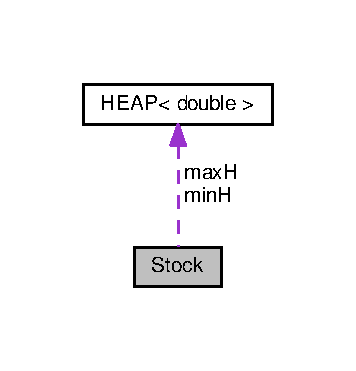
\includegraphics[width=171pt]{classStock__coll__graph}
\end{center}
\end{figure}
\subsubsection*{Public Member Functions}
\begin{DoxyCompactItemize}
\item 
\hyperlink{classStock_adddc4282213b3174a4299cca5a30117c}{Stock} ()
\end{DoxyCompactItemize}
\subsubsection*{Public Attributes}
\begin{DoxyCompactItemize}
\item 
\hyperlink{classHEAP}{H\+E\+A\+P}$<$ double $>$ \hyperlink{classStock_ab3a0f86a08ac6fa8dac1e9a1a855d0df}{min\+H}
\item 
\hyperlink{classHEAP}{H\+E\+A\+P}$<$ double $>$ \hyperlink{classStock_a00ba093f5066735943fc4651f17905fe}{max\+H}
\item 
std\+::string \hyperlink{classStock_a8b79c44538a5f8845a17e537798719e4}{name}
\end{DoxyCompactItemize}


\subsubsection{Detailed Description}
This is a class \hyperlink{classStock}{Stock} that creates min\+Heap and max\+Heap which are able to be called throughout the program. 

\subsubsection{Constructor \& Destructor Documentation}
\hypertarget{classStock_adddc4282213b3174a4299cca5a30117c}{\index{Stock@{Stock}!Stock@{Stock}}
\index{Stock@{Stock}!Stock@{Stock}}
\paragraph[{Stock}]{\setlength{\rightskip}{0pt plus 5cm}Stock\+::\+Stock (
\begin{DoxyParamCaption}
{}
\end{DoxyParamCaption}
)\hspace{0.3cm}{\ttfamily [inline]}}}\label{classStock_adddc4282213b3174a4299cca5a30117c}

\begin{DoxyCode}
9             : \hyperlink{classStock_ab3a0f86a08ac6fa8dac1e9a1a855d0df}{minH}(MAXHEAPSIZE,\hyperlink{classHEAP}{HEAP<double>::MIN}),
10               \hyperlink{classStock_a00ba093f5066735943fc4651f17905fe}{maxH}(MAXHEAPSIZE,\hyperlink{classHEAP}{HEAP<double>::MAX}) \{\}
\end{DoxyCode}


\subsubsection{Member Data Documentation}
\hypertarget{classStock_a00ba093f5066735943fc4651f17905fe}{\index{Stock@{Stock}!max\+H@{max\+H}}
\index{max\+H@{max\+H}!Stock@{Stock}}
\paragraph[{max\+H}]{\setlength{\rightskip}{0pt plus 5cm}{\bf H\+E\+A\+P}$<$double$>$ Stock\+::max\+H}}\label{classStock_a00ba093f5066735943fc4651f17905fe}
\hypertarget{classStock_ab3a0f86a08ac6fa8dac1e9a1a855d0df}{\index{Stock@{Stock}!min\+H@{min\+H}}
\index{min\+H@{min\+H}!Stock@{Stock}}
\paragraph[{min\+H}]{\setlength{\rightskip}{0pt plus 5cm}{\bf H\+E\+A\+P}$<$double$>$ Stock\+::min\+H}}\label{classStock_ab3a0f86a08ac6fa8dac1e9a1a855d0df}
\hypertarget{classStock_a8b79c44538a5f8845a17e537798719e4}{\index{Stock@{Stock}!name@{name}}
\index{name@{name}!Stock@{Stock}}
\paragraph[{name}]{\setlength{\rightskip}{0pt plus 5cm}std\+::string Stock\+::name}}\label{classStock_a8b79c44538a5f8845a17e537798719e4}


The documentation for this class was generated from the following file\+:\begin{DoxyCompactItemize}
\item 
\hyperlink{Stock_8h}{Stock.\+h}\end{DoxyCompactItemize}

\section{File Documentation}
\hypertarget{HEAP_8H}{\subsection{H\+E\+A\+P.\+H File Reference}
\label{HEAP_8H}\index{H\+E\+A\+P.\+H@{H\+E\+A\+P.\+H}}
}
{\ttfamily \#include $<$cctype$>$}\\*
{\ttfamily \#include $<$string.\+h$>$}\\*
{\ttfamily \#include $<$fstream$>$}\\*
{\ttfamily \#include $<$iostream$>$}\\*
{\ttfamily \#include $<$vector$>$}\\*
{\ttfamily \#include $<$sstream$>$}\\*
{\ttfamily \#include $<$string$>$}\\*
Include dependency graph for H\+E\+A\+P.\+H\+:\nopagebreak
\begin{figure}[H]
\begin{center}
\leavevmode
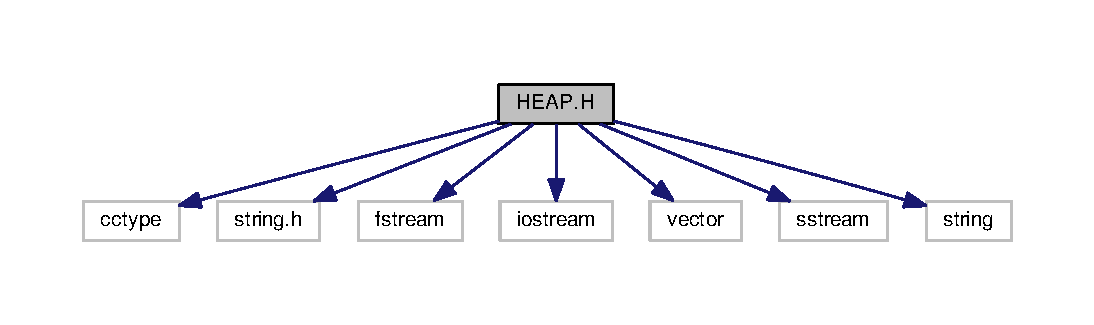
\includegraphics[width=350pt]{HEAP_8H__incl}
\end{center}
\end{figure}
This graph shows which files directly or indirectly include this file\+:\nopagebreak
\begin{figure}[H]
\begin{center}
\leavevmode
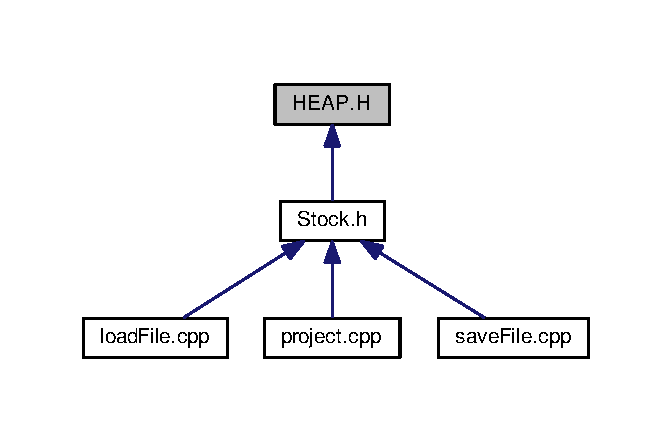
\includegraphics[width=322pt]{HEAP_8H__dep__incl}
\end{center}
\end{figure}
\subsubsection*{Classes}
\begin{DoxyCompactItemize}
\item 
class \hyperlink{classHEAP}{H\+E\+A\+P$<$ S\+O\+M\+E\+T\+Y\+P\+E $>$}
\begin{DoxyCompactList}\small\item\em This is a class \hyperlink{classHEAP}{H\+E\+A\+P} which includes all function and storage needed to make the program and tree. \end{DoxyCompactList}\end{DoxyCompactItemize}
\subsubsection*{Enumerations}
\begin{DoxyCompactItemize}
\item 
enum \hyperlink{HEAP_8H_a32c27cc471df37f4fc818d65de0a56c4}{S\+T\+A\+T\+U\+S} \{ \hyperlink{HEAP_8H_a32c27cc471df37f4fc818d65de0a56c4a2bc49ec37d6a5715dd23e85f1ff5bb59}{O\+K}, 
\hyperlink{HEAP_8H_a32c27cc471df37f4fc818d65de0a56c4aecedb56d1405a60c6069f4a0139bdec5}{F\+A\+I\+L\+E\+D}
 \}
\begin{DoxyCompactList}\small\item\em This is an enumeration that adds a status for O\+K and F\+A\+I\+L\+E\+D instead of true and false boolean. \end{DoxyCompactList}\end{DoxyCompactItemize}
\subsubsection*{Functions}
\begin{DoxyCompactItemize}
\item 
{\footnotesize template$<$class S\+O\+M\+E\+T\+Y\+P\+E $>$ }\\void \hyperlink{classHEAP}{H\+E\+A\+P}$<$ S\+O\+M\+E\+T\+Y\+P\+E $>$\+::void \hyperlink{HEAP_8H_ac4a84c5d4f565cec7c43b7a43d4aec9d}{add\+Max\+H\+V} (int value)
\begin{DoxyCompactList}\small\item\em This adds the value into the max\+Heap vector. \end{DoxyCompactList}\end{DoxyCompactItemize}


\subsubsection{Enumeration Type Documentation}
\hypertarget{HEAP_8H_a32c27cc471df37f4fc818d65de0a56c4}{\index{H\+E\+A\+P.\+H@{H\+E\+A\+P.\+H}!S\+T\+A\+T\+U\+S@{S\+T\+A\+T\+U\+S}}
\index{S\+T\+A\+T\+U\+S@{S\+T\+A\+T\+U\+S}!H\+E\+A\+P.\+H@{H\+E\+A\+P.\+H}}
\paragraph[{S\+T\+A\+T\+U\+S}]{\setlength{\rightskip}{0pt plus 5cm}enum {\bf S\+T\+A\+T\+U\+S}}}\label{HEAP_8H_a32c27cc471df37f4fc818d65de0a56c4}


This is an enumeration that adds a status for O\+K and F\+A\+I\+L\+E\+D instead of true and false boolean. 

\begin{Desc}
\item[Enumerator]\par
\begin{description}
\index{O\+K@{O\+K}!H\+E\+A\+P.\+H@{H\+E\+A\+P.\+H}}\index{H\+E\+A\+P.\+H@{H\+E\+A\+P.\+H}!O\+K@{O\+K}}\item[{\em 
\hypertarget{HEAP_8H_a32c27cc471df37f4fc818d65de0a56c4a2bc49ec37d6a5715dd23e85f1ff5bb59}{O\+K}\label{HEAP_8H_a32c27cc471df37f4fc818d65de0a56c4a2bc49ec37d6a5715dd23e85f1ff5bb59}
}]\index{F\+A\+I\+L\+E\+D@{F\+A\+I\+L\+E\+D}!H\+E\+A\+P.\+H@{H\+E\+A\+P.\+H}}\index{H\+E\+A\+P.\+H@{H\+E\+A\+P.\+H}!F\+A\+I\+L\+E\+D@{F\+A\+I\+L\+E\+D}}\item[{\em 
\hypertarget{HEAP_8H_a32c27cc471df37f4fc818d65de0a56c4aecedb56d1405a60c6069f4a0139bdec5}{F\+A\+I\+L\+E\+D}\label{HEAP_8H_a32c27cc471df37f4fc818d65de0a56c4aecedb56d1405a60c6069f4a0139bdec5}
}]\end{description}
\end{Desc}

\begin{DoxyCode}
18 \{\hyperlink{HEAP_8H_a32c27cc471df37f4fc818d65de0a56c4a2bc49ec37d6a5715dd23e85f1ff5bb59}{OK},\hyperlink{HEAP_8H_a32c27cc471df37f4fc818d65de0a56c4aecedb56d1405a60c6069f4a0139bdec5}{FAILED}\};
\end{DoxyCode}


\subsubsection{Function Documentation}
\hypertarget{HEAP_8H_ac4a84c5d4f565cec7c43b7a43d4aec9d}{\index{H\+E\+A\+P.\+H@{H\+E\+A\+P.\+H}!add\+Max\+H\+V@{add\+Max\+H\+V}}
\index{add\+Max\+H\+V@{add\+Max\+H\+V}!H\+E\+A\+P.\+H@{H\+E\+A\+P.\+H}}
\paragraph[{add\+Max\+H\+V}]{\setlength{\rightskip}{0pt plus 5cm}template$<$class S\+O\+M\+E\+T\+Y\+P\+E $>$ void {\bf H\+E\+A\+P}$<$S\+O\+M\+E\+T\+Y\+P\+E$>$\+::void add\+Max\+H\+V (
\begin{DoxyParamCaption}
\item[{int}]{value}
\end{DoxyParamCaption}
)}}\label{HEAP_8H_ac4a84c5d4f565cec7c43b7a43d4aec9d}


This adds the value into the max\+Heap vector. 


\begin{DoxyParams}{Parameters}
{\em a} & value of int to be added into max\+Heap \\
\hline
\end{DoxyParams}

\begin{DoxyCode}
94 \{
95     maxHV.push\_back(value);
96 \}
\end{DoxyCode}

\hypertarget{loadFile_8cpp}{\subsection{load\+File.\+cpp File Reference}
\label{loadFile_8cpp}\index{load\+File.\+cpp@{load\+File.\+cpp}}
}
{\ttfamily \#include \char`\"{}Stock.\+h\char`\"{}}\\*
Include dependency graph for load\+File.\+cpp\+:\nopagebreak
\begin{figure}[H]
\begin{center}
\leavevmode
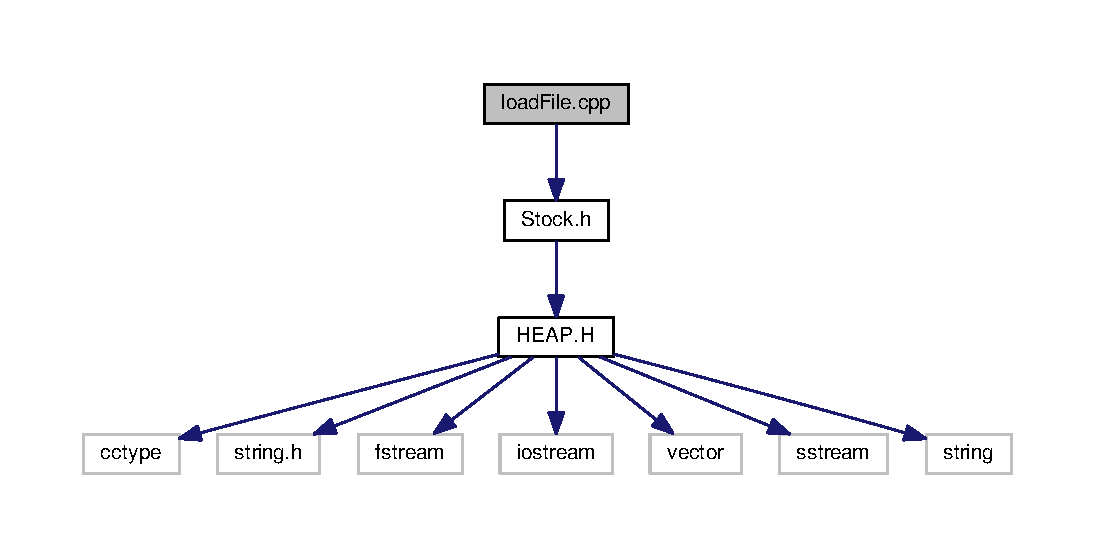
\includegraphics[width=350pt]{loadFile_8cpp__incl}
\end{center}
\end{figure}
\subsubsection*{Functions}
\begin{DoxyCompactItemize}
\item 
void \hyperlink{loadFile_8cpp_aa059384bbb4de4156d602a4293d88ef4}{load\+File} (std\+::string f, std\+::vector$<$ double $>$ \&v)
\begin{DoxyCompactList}\small\item\em This is a function that loads a text file with information of the heap trees. \end{DoxyCompactList}\end{DoxyCompactItemize}


\subsubsection{Function Documentation}
\hypertarget{loadFile_8cpp_aa059384bbb4de4156d602a4293d88ef4}{\index{load\+File.\+cpp@{load\+File.\+cpp}!load\+File@{load\+File}}
\index{load\+File@{load\+File}!load\+File.\+cpp@{load\+File.\+cpp}}
\paragraph[{load\+File}]{\setlength{\rightskip}{0pt plus 5cm}void load\+File (
\begin{DoxyParamCaption}
\item[{std\+::string}]{f, }
\item[{std\+::vector$<$ double $>$ \&}]{v}
\end{DoxyParamCaption}
)}}\label{loadFile_8cpp_aa059384bbb4de4156d602a4293d88ef4}


This is a function that loads a text file with information of the heap trees. 


\begin{DoxyParams}{Parameters}
{\em string} & to write in the file and a vector to reference the info that will be loaded from the file \\
\hline
\end{DoxyParams}
\begin{DoxyReturn}{Returns}
return information 
\end{DoxyReturn}

\begin{DoxyCode}
3                                                  \{
4     std::ifstream ifs(f);
5     \textcolor{keywordtype}{double} x;
6     \textcolor{keywordflow}{while}(ifs >> x) \{
7         \textcolor{comment}{//std::cout << "From file: " << x << std::endl;}
8         v.push\_back(x);
9     \}
10     ifs.close();
11 \}
\end{DoxyCode}

\hypertarget{project_8cpp}{\subsection{project.\+cpp File Reference}
\label{project_8cpp}\index{project.\+cpp@{project.\+cpp}}
}
{\ttfamily \#include \char`\"{}Stock.\+h\char`\"{}}\\*
Include dependency graph for project.\+cpp\+:\nopagebreak
\begin{figure}[H]
\begin{center}
\leavevmode
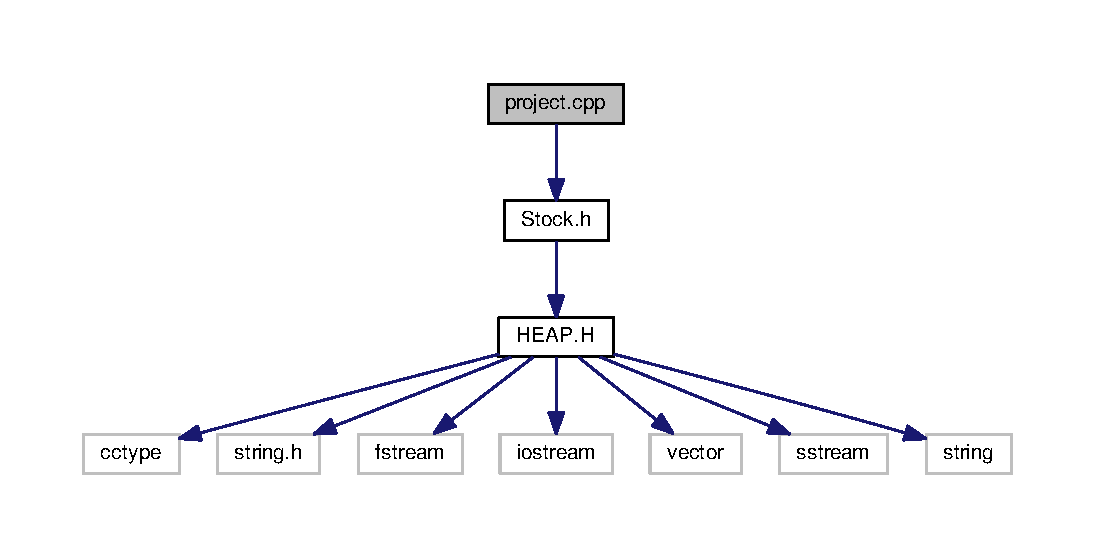
\includegraphics[width=350pt]{project_8cpp__incl}
\end{center}
\end{figure}
\subsubsection*{Functions}
\begin{DoxyCompactItemize}
\item 
int \hyperlink{project_8cpp_ae66f6b31b5ad750f1fe042a706a4e3d4}{main} ()
\end{DoxyCompactItemize}


\subsubsection{Function Documentation}
\hypertarget{project_8cpp_ae66f6b31b5ad750f1fe042a706a4e3d4}{\index{project.\+cpp@{project.\+cpp}!main@{main}}
\index{main@{main}!project.\+cpp@{project.\+cpp}}
\paragraph[{main}]{\setlength{\rightskip}{0pt plus 5cm}int main (
\begin{DoxyParamCaption}
{}
\end{DoxyParamCaption}
)}}\label{project_8cpp_ae66f6b31b5ad750f1fe042a706a4e3d4}

\begin{DoxyCode}
3 \{    
4     \hyperlink{classStock}{Stock} s;
5     std::vector<double> v;
6     std::vector<double> z;
7     std::string test = getenv(\textcolor{stringliteral}{"QUERY\_STRING"});
8     std::string delimiter = \textcolor{stringliteral}{"&"};
9     std::string stockName = test.substr(0, test.find(delimiter)); \textcolor{comment}{// extract StockName}
10     test.erase(0, stockName.length()+1); \textcolor{comment}{// Remove Stock Info from string}
11     stockName.erase(0,6);
12     std::string typeInput = test.substr(0, test.find(delimiter));
13     test.erase(0, typeInput.length()+1);
14     typeInput.erase(0,2);
15     std::string nameInput = test.substr(0, test.find(delimiter));
16     test.erase(0, nameInput.length()+1);
17     nameInput.erase(0,2);
18     std::string sharesInput = test.substr(0, test.find(delimiter));
19     test.erase(0, sharesInput.length());
20     sharesInput.erase(0,2);
21     std::string priceInput = test;
22     priceInput.erase(0,3);
23     \textcolor{comment}{/*}
24 \textcolor{comment}{    std::cout << priceInput << std::endl;}
25 \textcolor{comment}{    std::cout << "*****************" << std::endl;}
26 \textcolor{comment}{    std::cout << stockName << std::endl;}
27 \textcolor{comment}{    std::cout << typeInput << std::endl;}
28 \textcolor{comment}{    std::cout << nameInput << std::endl;}
29 \textcolor{comment}{    std::cout << sharesInput << std::endl;}
30 \textcolor{comment}{    std::cout << priceInput << std::endl;}
31 \textcolor{comment}{    std::cout << "**************" << std::endl;}
32 \textcolor{comment}{    */}
33     \textcolor{keywordflow}{if} (typeInput == \textcolor{stringliteral}{"Buy"}) \{
34         \textcolor{keywordtype}{double} priceDouble = std::stod(priceInput);
35         s.\hyperlink{classStock_a00ba093f5066735943fc4651f17905fe}{maxH}.\hyperlink{classHEAP_a61daf2c080cdb92947a0e591fbd8d772}{Insert}(priceDouble);
36         s.\hyperlink{classStock_a00ba093f5066735943fc4651f17905fe}{maxH}.\hyperlink{classHEAP_a61daf2c080cdb92947a0e591fbd8d772}{Insert}(priceDouble);
37         \textcolor{comment}{//s.maxH.printHeap();}
38         \textcolor{keywordtype}{double} shareDouble = std::stod(sharesInput);
39         \textcolor{comment}{//std::cout << "priceDouble: " << priceDouble << std::endl;}
40         \textcolor{comment}{//std::cout << "shareDouble: " <<  shareDouble << std::endl;}
41         \hyperlink{loadFile_8cpp_aa059384bbb4de4156d602a4293d88ef4}{loadFile}(\textcolor{stringliteral}{"/home/debian/cs124/stock/shares.json"}, z); 
42         \hyperlink{loadFile_8cpp_aa059384bbb4de4156d602a4293d88ef4}{loadFile}(\textcolor{stringliteral}{"/home/debian/cs124/stock/min.json"}, v);
43         \textcolor{comment}{//std::cout << v[0] << std::endl;}
44         \textcolor{keywordflow}{if} (v.size() == 0 )
45             std::cout << \textcolor{stringliteral}{"<html><h1>No seller found. Request pending...</h1></html>"} << std::endl;
46         \textcolor{keywordflow}{else} \textcolor{keywordflow}{if}(v.size() != 0 ) \{
47             \textcolor{keywordtype}{int} i;
48             \textcolor{keywordflow}{for}(i = 0; i < v.size(); i++) \{
49                 \textcolor{keywordflow}{if} (priceDouble == v[i]) \{
50                     std::cout << \textcolor{stringliteral}{"<html><h1>Match found!</h1></html>"} << std::endl;
51                     shareDouble = shareDouble;
52                     std::cout << \textcolor{stringliteral}{"<html><h2>Stock: Nvidia<h2></html>"} << std::endl;
53                     std::cout << \textcolor{stringliteral}{"<html><h3>Name: Market</h3></html>"} << std::endl;
54                     std::cout << \textcolor{stringliteral}{"<html><h4>Shares:"} << shareDouble << \textcolor{stringliteral}{"</h4></html>"} << std::endl;
55                     std::cout << \textcolor{stringliteral}{"<html><h5>Type: Sell </h5></html>"} << std::endl;
56                     std::cout << \textcolor{stringliteral}{"<html><h6>Prices:"} << priceDouble << \textcolor{stringliteral}{"</h6></html>"} << std::endl;
57                 \}
58                 \textcolor{keywordflow}{if}(i == v.size()-1 && priceDouble != v[i])
59                     std::cout << \textcolor{stringliteral}{"<html><h1>No seller found. Request pending...</h1></html"} << std::endl;
60                 \}
61         \}
62         v.clear();
63         v.push\_back(priceDouble);
64         z.clear();
65         z.push\_back(shareDouble);
66         \hyperlink{saveFile_8cpp_ad613df1d9cfb29d70e453c5bdec4a9b8}{saveFile}(\textcolor{stringliteral}{"/home/debian/cs124/stock/info.json"}, v);
67         \hyperlink{saveFile_8cpp_ad613df1d9cfb29d70e453c5bdec4a9b8}{saveFile}(\textcolor{stringliteral}{"/home/debian/cs124/stock/shares.json"}, z);  
68     \}
69     \textcolor{keywordflow}{else} \textcolor{keywordflow}{if} (typeInput == \textcolor{stringliteral}{"Sell"}) \{
70         \textcolor{keywordtype}{double} priceDouble = std::stod(priceInput);
71         s.\hyperlink{classStock_ab3a0f86a08ac6fa8dac1e9a1a855d0df}{minH}.\hyperlink{classHEAP_a61daf2c080cdb92947a0e591fbd8d772}{Insert}(priceDouble);
72         s.\hyperlink{classStock_ab3a0f86a08ac6fa8dac1e9a1a855d0df}{minH}.\hyperlink{classHEAP_a61daf2c080cdb92947a0e591fbd8d772}{Insert}(priceDouble);
73         \textcolor{comment}{//s.minH.printHeap();}
74         \textcolor{keywordtype}{double} shareDouble = std::stod(sharesInput);
75         \textcolor{comment}{//std::cout << "sharesInput: " << sharesInput << std::endl;}
76         \textcolor{comment}{//std::cout << "priceDouble: " << priceDouble << std::endl;}
77         \hyperlink{loadFile_8cpp_aa059384bbb4de4156d602a4293d88ef4}{loadFile}(\textcolor{stringliteral}{"/home/debian/cs124/stock/shares.json"}, z);
78         \hyperlink{loadFile_8cpp_aa059384bbb4de4156d602a4293d88ef4}{loadFile}(\textcolor{stringliteral}{"/home/debian/cs124/stock/info.json"}, v);
79         \textcolor{keywordflow}{if} (v.size() == 0 )
80             std::cout << \textcolor{stringliteral}{"<html><h1>No seller found. Request pending...</h1></html>"} << std::endl;
81         \textcolor{keywordflow}{else} \textcolor{keywordflow}{if}(v.size() != 0 ) \{
82             \textcolor{keywordtype}{int} i;
83             \textcolor{keywordflow}{for}(i = 0; i < v.size(); i++) \{
84                 \textcolor{keywordflow}{if} (priceDouble == v[i]) \{
85                     shareDouble = shareDouble;
86                     \textcolor{keywordflow}{if}( shareDouble < 0) 
87                         shareDouble = shareDouble * -1;
88                     std::cout << \textcolor{stringliteral}{"<html><h1>Match found!</h1></html>"} << std::endl;
89                     std::cout << \textcolor{stringliteral}{"<html><h2>Stock: Nvidia<h2></html>"} << std::endl;
90                     std::cout << \textcolor{stringliteral}{"<html><h3>Name: Market</h3></html>"} << std::endl;
91                     std::cout << \textcolor{stringliteral}{"<html><h4>Shares:"} << shareDouble << \textcolor{stringliteral}{"</h4></html>"} << std::endl;
92                     std::cout << \textcolor{stringliteral}{"<html><h5>Type: Buy </h5></html>"} << std::endl;
93                     std::cout << \textcolor{stringliteral}{"<html><h6>Prices:"} << priceDouble << \textcolor{stringliteral}{"</h6></html>"} << std::endl;
94                 \}
95                 \textcolor{keywordflow}{if}(i == v.size()-1 && priceDouble != v[i])
96                     std::cout << \textcolor{stringliteral}{"<html><h1>No buyer found. Request pending...</h1></html>"} << std::endl;
97                 \}
98         \}
99         v.clear();
100         v.push\_back(priceDouble);
101         z.clear();
102         z.push\_back(shareDouble);
103         \hyperlink{saveFile_8cpp_ad613df1d9cfb29d70e453c5bdec4a9b8}{saveFile}(\textcolor{stringliteral}{"/home/debian/cs124/stock/min.json"}, v);
104         \hyperlink{saveFile_8cpp_ad613df1d9cfb29d70e453c5bdec4a9b8}{saveFile}(\textcolor{stringliteral}{"/home/debian/cs124/stock/shares.json"}, z);    
105         \}
106 \}
\end{DoxyCode}

\hypertarget{saveFile_8cpp}{\subsection{save\+File.\+cpp File Reference}
\label{saveFile_8cpp}\index{save\+File.\+cpp@{save\+File.\+cpp}}
}
{\ttfamily \#include \char`\"{}Stock.\+h\char`\"{}}\\*
Include dependency graph for save\+File.\+cpp\+:\nopagebreak
\begin{figure}[H]
\begin{center}
\leavevmode
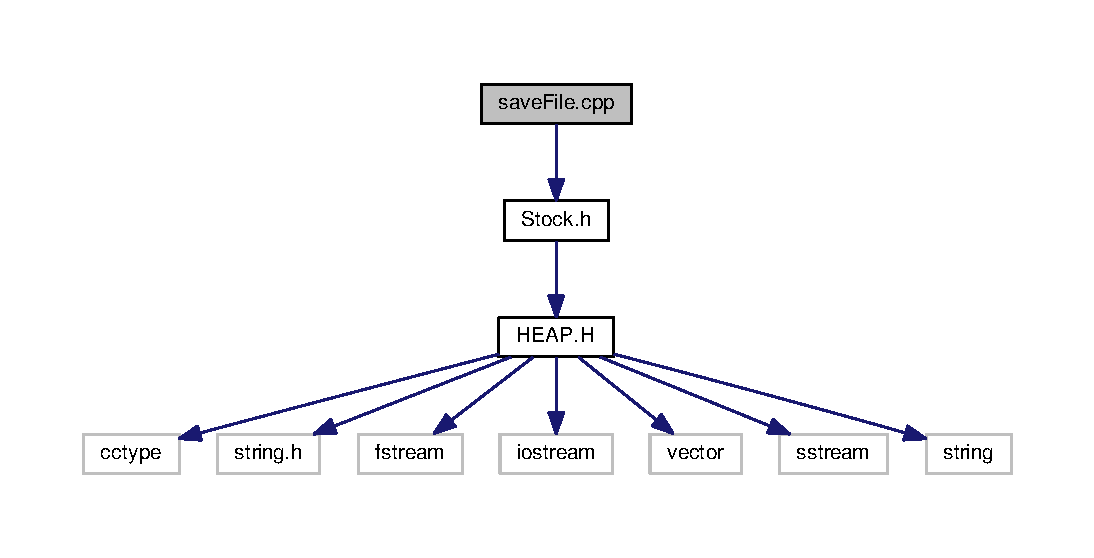
\includegraphics[width=350pt]{saveFile_8cpp__incl}
\end{center}
\end{figure}
\subsubsection*{Functions}
\begin{DoxyCompactItemize}
\item 
void \hyperlink{saveFile_8cpp_ad613df1d9cfb29d70e453c5bdec4a9b8}{save\+File} (std\+::string f, std\+::vector$<$ double $>$ \&v)
\begin{DoxyCompactList}\small\item\em This is a function that saves into a text file with the user's information. \end{DoxyCompactList}\end{DoxyCompactItemize}


\subsubsection{Function Documentation}
\hypertarget{saveFile_8cpp_ad613df1d9cfb29d70e453c5bdec4a9b8}{\index{save\+File.\+cpp@{save\+File.\+cpp}!save\+File@{save\+File}}
\index{save\+File@{save\+File}!save\+File.\+cpp@{save\+File.\+cpp}}
\paragraph[{save\+File}]{\setlength{\rightskip}{0pt plus 5cm}void save\+File (
\begin{DoxyParamCaption}
\item[{std\+::string}]{f, }
\item[{std\+::vector$<$ double $>$ \&}]{v}
\end{DoxyParamCaption}
)}}\label{saveFile_8cpp_ad613df1d9cfb29d70e453c5bdec4a9b8}


This is a function that saves into a text file with the user's information. 


\begin{DoxyParams}{Parameters}
{\em string} & to write in the file and a vector to reference the info that will be saved into the file \\
\hline
\end{DoxyParams}

\begin{DoxyCode}
3                                                  \{
4     std::ofstream ofs;
5     ofs.open(f);
6     \textcolor{keywordflow}{for}(\textcolor{keywordtype}{int} i = 0; i < v.size(); i++) \{
7         \textcolor{comment}{//std::cout << "Save File: " << v[i] << std::endl;}
8         ofs << v[i];
9     \}
10     ofs.close();
11 \}
\end{DoxyCode}

\hypertarget{stock_8dox}{\subsection{stock.\+dox File Reference}
\label{stock_8dox}\index{stock.\+dox@{stock.\+dox}}
}

\hypertarget{Stock_8h}{\subsection{Stock.\+h File Reference}
\label{Stock_8h}\index{Stock.\+h@{Stock.\+h}}
}
{\ttfamily \#include \char`\"{}H\+E\+A\+P.\+H\char`\"{}}\\*
Include dependency graph for Stock.\+h\+:\nopagebreak
\begin{figure}[H]
\begin{center}
\leavevmode
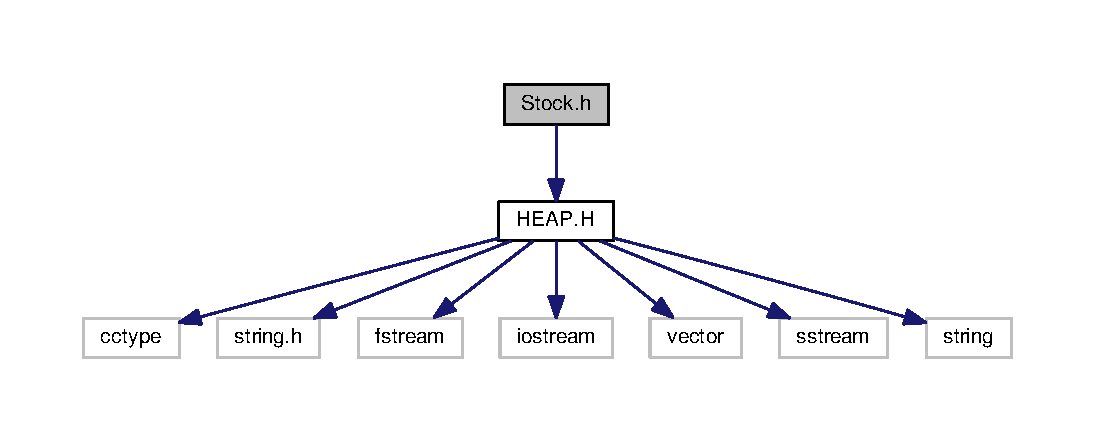
\includegraphics[width=350pt]{Stock_8h__incl}
\end{center}
\end{figure}
This graph shows which files directly or indirectly include this file\+:\nopagebreak
\begin{figure}[H]
\begin{center}
\leavevmode
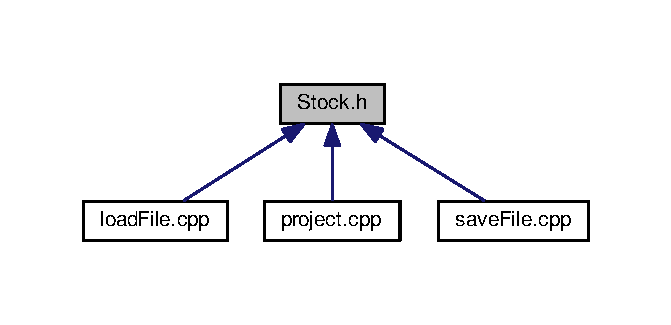
\includegraphics[width=322pt]{Stock_8h__dep__incl}
\end{center}
\end{figure}
\subsubsection*{Classes}
\begin{DoxyCompactItemize}
\item 
class \hyperlink{classStock}{Stock}
\begin{DoxyCompactList}\small\item\em This is a class \hyperlink{classStock}{Stock} that creates min\+Heap and max\+Heap which are able to be called throughout the program. \end{DoxyCompactList}\end{DoxyCompactItemize}
\subsubsection*{Functions}
\begin{DoxyCompactItemize}
\item 
void \hyperlink{Stock_8h_aa059384bbb4de4156d602a4293d88ef4}{load\+File} (std\+::string f, std\+::vector$<$ double $>$ \&v)
\begin{DoxyCompactList}\small\item\em This is a function that loads a text file with information of the heap trees. \end{DoxyCompactList}\item 
void \hyperlink{Stock_8h_ad613df1d9cfb29d70e453c5bdec4a9b8}{save\+File} (std\+::string f, std\+::vector$<$ double $>$ \&v)
\begin{DoxyCompactList}\small\item\em This is a function that saves into a text file with the user's information. \end{DoxyCompactList}\end{DoxyCompactItemize}


\subsubsection{Function Documentation}
\hypertarget{Stock_8h_aa059384bbb4de4156d602a4293d88ef4}{\index{Stock.\+h@{Stock.\+h}!load\+File@{load\+File}}
\index{load\+File@{load\+File}!Stock.\+h@{Stock.\+h}}
\paragraph[{load\+File}]{\setlength{\rightskip}{0pt plus 5cm}void load\+File (
\begin{DoxyParamCaption}
\item[{std\+::string}]{f, }
\item[{std\+::vector$<$ double $>$ \&}]{v}
\end{DoxyParamCaption}
)}}\label{Stock_8h_aa059384bbb4de4156d602a4293d88ef4}


This is a function that loads a text file with information of the heap trees. 


\begin{DoxyParams}{Parameters}
{\em string} & to write in the file and a vector to reference the info that will be loaded from the file \\
\hline
\end{DoxyParams}
\begin{DoxyReturn}{Returns}
return information 
\end{DoxyReturn}

\begin{DoxyCode}
3                                                  \{
4     std::ifstream ifs(f);
5     \textcolor{keywordtype}{double} x;
6     \textcolor{keywordflow}{while}(ifs >> x) \{
7         \textcolor{comment}{//std::cout << "From file: " << x << std::endl;}
8         v.push\_back(x);
9     \}
10     ifs.close();
11 \}
\end{DoxyCode}
\hypertarget{Stock_8h_ad613df1d9cfb29d70e453c5bdec4a9b8}{\index{Stock.\+h@{Stock.\+h}!save\+File@{save\+File}}
\index{save\+File@{save\+File}!Stock.\+h@{Stock.\+h}}
\paragraph[{save\+File}]{\setlength{\rightskip}{0pt plus 5cm}void save\+File (
\begin{DoxyParamCaption}
\item[{std\+::string}]{f, }
\item[{std\+::vector$<$ double $>$ \&}]{v}
\end{DoxyParamCaption}
)}}\label{Stock_8h_ad613df1d9cfb29d70e453c5bdec4a9b8}


This is a function that saves into a text file with the user's information. 


\begin{DoxyParams}{Parameters}
{\em string} & to write in the file and a vector to reference the info that will be saved into the file \\
\hline
\end{DoxyParams}

\begin{DoxyCode}
3                                                  \{
4     std::ofstream ofs;
5     ofs.open(f);
6     \textcolor{keywordflow}{for}(\textcolor{keywordtype}{int} i = 0; i < v.size(); i++) \{
7         \textcolor{comment}{//std::cout << "Save File: " << v[i] << std::endl;}
8         ofs << v[i];
9     \}
10     ofs.close();
11 \}
\end{DoxyCode}

%--- End generated contents ---

% Index
\newpage
\phantomsection
\addcontentsline{toc}{section}{Index}
\printindex

\end{document}
